\documentclass[a4paper,11pt]{article}%Schriftgröße

\usepackage[T1]{fontenc} 
\usepackage[utf8]{inputenc}
\usepackage[ngerman]{babel}%Veröffentlichungssprache
\usepackage{graphicx}
\usepackage{ragged2e}
\usepackage[format=plain,justification=RaggedRight,singlelinecheck=false,font={small},labelsep=space]{caption}
\usepackage{float}
\usepackage{xcolor}	
\usepackage[a4paper]{geometry}
\usepackage{fancyhdr}
\usepackage[onehalfspacing]{setspace}%Zeilenabstand
\usepackage[onehalfspacing]{setspace}%Zeilenabstand
\usepackage{fancyhdr}
\usepackage[authoryear]{natbib}
\usepackage[colorlinks,pdfpagelabels,pdfstartview = FitH,bookmarksopen = true,bookmarksnumbered = true,linkcolor = black,urlcolor = black,plainpages = false,hypertexnames = false,citecolor = black] {hyperref}
\usepackage[printonlyused, withpage, smaller]{acronym}
\renewcommand{\\}{\vspace*{0.5\baselineskip} \newline}
\renewcommand*\MakeUppercase[1]{#1}	
\renewcommand{\familydefault}{\sfdefault}
\geometry{left=3.5cm,right=2.5cm,top=2.4cm,bottom=2cm}%Seitenränder
\pagestyle{fancy}
\renewcommand{\headrulewidth}{0pt}
\renewcommand{\footrulewidth}{0pt}
\fancyhead[R]{\footnotesize{\thepage}}
\fancyhead[L]{\footnotesize{\leftmark}}
\fancyfoot{}

\begin{document}
	\begin{titlepage}
		\begin{flushleft}
			\vspace*{-1cm}
			
\includegraphics[scale=1]{Abbildungen/TH.png}\\
			\vspace*{1cm}
		\end{flushleft}
		
		\begin{huge}
			\noindent
			%Vergleich des Teambuildingerfolgs mittels eines nicht-vollkörpergetracktem- und vollkörpergetracktem Avatars in einer Immersive Virtual Reality anhand einer Escape-Room-Artigen Umgebung. \\
			
%			Vertrauensaufbau einer Teambuildingmaßnahme zwischen eines Hand- und Kopf getracktem Avatar und  eines Hand-, Kopf und Inverskinematisch-simuliertem Torsos getracktem Avatar in einem Shared Virtual Environment anhand einer Escape-Room-Artigen Umgebung. \\
			
%			Auswirkung des Vertrauens auf die Effizienz in einer Teambuildingmaßnahme anhand eines Hand- und Kopfgetracktem und einem Hand-, Kopf und Inverskinematisch-simuliertem Torsos getracktem Avatar ein einem Shared Virtual Environment. //
			
%			Auswirkung von Vertrauen zu Avataren auf die \mbox{Effizienz} in einer Teambuildingmaßnahme in ein einem Shared Virtual Environment.

Auswirkung des Vertrauens auf die Effizienz in einer Teambuildingmaßnahme anhand eines \flqq IK-Avatar\flqq und einem \flqq Non-IK-Avatar\frqq in einem Shared-Virtual-Environment. \\
		\end{huge}
		
		Masterarbeit zur Erlangung des Master-Grades \newline
		\textit{Master of Science} im Studiengang Medientechnologie \newline
		an der Fakultät für Informations-, Medien- und Elektrotechnik \newline
		der Technischen Hochschule Köln \\
		~\\
		~\\
		~\\
		\noindent\begin{tabular}{ll}
			vorgelegt von: & Hannes Hinrichs \\
			Matrikel-Nr.: &	11121733 \\
			Adresse: & Zülpicher Straße 19 \\
			~ &	50674 Köln \\
			~ &	hannes.hinrichs@web.de \\
			~ & ~ \\
			eingereicht bei: & Prof. Dr. Arnulph Fuhrmann \\
			Zweitgutachter/in: & --------------------
		\end{tabular}	
		~\\
		~\\
		Ort, TT.MM.JJJJ
	\end{titlepage}
	\pagenumbering{Roman}
	\pagestyle{fancy}
	\newpage
	\section*{Erklärung}\markboth{Erklärung}{Erklärung}\addcontentsline{toc}{section}{Erklärung}
	Ich versichere, die von mir vorgelegte Arbeit selbstständig verfasst zu haben. Alle Stellen, die wörtlich oder sinngemäß aus veröffentlichten oder nicht veröffentlichten Arbeiten anderer oder der Verfasserin/des Verfassers selbst entnommen sind, habe ich als entnommen kenntlich gemacht. Sämtliche Quellen und Hilfsmittel, die ich für die Arbeit benutzt habe, sind angegeben. Die Arbeit hat mit gleichem Inhalt bzw. in wesentlichen Teilen noch keiner anderen Prüfungsbehörde vorgelegen.\\
	Anmerkung: In einigen Studiengängen steht die Erklärung am Ende des Textes.\\
	~\\
	~\\
	\rule{0.35\textwidth}{0.4pt} \hspace*{3cm} \rule{0.45\textwidth}{0.4pt} \newline
	Ort, Datum	\hspace*{6.3cm}	Rechtsverbindliche Unterschrift
	\newpage
	\section*{Kurzfassung/Abstract}\markboth{Kurzfassung/Abstract}{Kurzfassung/Abstract}\addcontentsline{toc}{section}{Kurzfassung/Abstract}
	Virtual Reality \ac{vr} hat in den letzten Jahren aufgrund von verbesserter Technologie und sinkenden Kosten an bedeutung gewonnen. Verschiedene Felder, wie Medizin, Wirtschaft, Training oder die Industrie greifen auf diese Technologie zurück. Vorranschreitende Forschung in diesem Feld, ist aufgrund von wachsendem Interesse von großer Bedeutung. Vertrauensbildung und das gesamte Konstrukt von Vertrauen ist in vielen Feldern eine wichtige Grundlage, wurde in der Forschung im Zusammenhang mit \ac{vr} jedoch in den letzten Jahren wenig betrieben. Diese Arbeit zielt darauf ab, das Konstrukt des Vertrauens in der Virtuellen Welt besser zu verstehen und mit diesem umzugehen. Dafür wurde eine Studie der Technischen Hochschule zu Köln durchgeführt, um einen Zusammenhang der Vertrauensbildung in einer Teambuildingmaßnahme zwischen einem Menschenähnlichen Avatar und einem nicht-Menschenähnlichen Avatar, darzustellen.
	
	\paragraph{Virtual-Reality, Vertrauen, Teambuilding, Avatar}
	\newpage
	\tableofcontents
	\newpage
	
	\section*{Abkürzungsverzeichnis}\markboth{Abkürzungsverzeichnis}{Abkürzungsverzeichnis}\addcontentsline{toc}{section}{Abkürzungsverzeichnis}
	\begin{acronym}[NIK-T.Lvl.Rounds]
	\acro{hmd}[HMD]{Head-Mounted-Display}
	\acro{sve}[SVE]{Shared-Virtual-Environment}
	\acro{vr}[VR]{Virtual-Reality}
	\acro{ivr}[IVR]{Immersive-Virtual-Reality}
	\acro{ipo}[IPO]{Input-Process-Output}
	\acro{fov}[FOV]{Field-of-View}
	\acro{bip}[BIP]{Break-in-Presence}
	
	\acro{ik}[IK]{Invers-Kinematisch - (Hand-, Kopf und Inverskinematisch-simulierter Torso)}
	\acro{nik}[NIK]{Nicht-Invers-Kinematisch (Hand- und Kopf getrackter Avatar)}
	
	\acro{gt}[GT]{Generelles Vertrauen}
	\acro{gti}[GTI]{Generelles Vertrauen - IK}
	\acro{gtn}[GTN]{Generelles Vertrauen - NIK}
	
	\acro{ct}[CT]{Kognitives Vertrauen}
	\acro{cti}[CTI]{Kognitives Vertrauen - IK}
	\acro{ctn}[CTN]{Kognitives Vertrauen - NIK}
	
	\acro{tc}[TC]{Team-Kommunikation}
	\acro{tci}[TCI]{Team-Kommunikation - IK}
	\acro{tcn}[TCN]{Team-Kommunikation - NIK}
	
	\acro{tRound}[T.Lvl.Rounds]{Erfolgreich abgeschlossene Runden auf Team-Level}
	\acro{tRoundIK}[IK-T.Lvl.Rounds]{Erfolgreiche abgeschlossene Runden auf Team-Level - IK}
	\acro{tRoundNIK}[NIK-T.Lvl.Rounds]{Erfolgreiche abgeschlossene Runden auf Team-Level - NIK}
	
	\acro{te}[TE]{Teameffektivität}
	\acro{tei}[TEI]{Teameffektivität - IK}
	\acro{ten}[TEN]{Teameffektivität - NIK}
	
	\acro{cp}[CP]{Co-Präsenz}
	\acro{cpi}[CPI]{Co-Präsenz - IK}
	\acro{cpn}[CPN]{Co-Präsenz - NIK}
	
	\acro{tlx}[NTLX]{Nasa-TLX}
	\acro{tlxi}[NTLXI]{Nasa-TLX - IK}
	\acro{tlxn}[NTLXN]{Nasa-TLX - NIK}
	
	\acro{teamCog}[T.Lvl.Cog]{Kognitives Vertrauen auf Team-Level}
	\acro{teamCogIK}[IK-T.Lvl.Cog]{Kognitives Vertrauen auf Team-Level - IK}
	\acro{teamCogNIK}[NIK-T.Lvl.Cog]{Kognitives Vertrauen auf Team-Level - NIK}
	
	\acro{teamGen}[T.Lvl.Gen]{Generelles Vertrauen auf Team-Level}
	\acro{teamGenIK}[IK-T.Lvl.Gen]{Generelles Vertrauen auf Team-Level - IK}
	\acro{teamGenNIK}[NIK-T.Lvl.Gen]{Generelles Vertrauen auf Team-Level - NIK}
	
	\acro{scp}[SCP]{Self-Co-Präsenz}
	\acro{scpi}[SCPI]{Self-Co-Präsenz - IK}
	\acro{scpn}[SCPN]{Self-Co-Präsenz - NIK}	
	
	\acro{ocp}[OCP]{Other-Co-Präsenz}
	\acro{ocpi}[OCPI]{Other-Co-Präsenz - IK}
	\acro{ocpn}[OCPN]{Other-Co-Präsenz - NIK}	
	
	\acro{ipq}[IPQ]{Fragebogen des Anstrengungsmaß}
	\acro{ipqi}[IPQI]{Fragebogen des Anstrengungsmaß - IK}
	\acro{ipqn}[IPQN]{Fragebogen des Anstrengungsmaß - NIK}
	
	\acro{tp}[TP]{Telepresence}
	\acro{tpi}[TPI]{Telepresence - IK}
	\acro{tpn}[TPN]{Telepresence - NIK}	
	
	\acro{sp}[SP]{Social-Presence}
	\acro{spi}[SPI]{Social-Presence - IK}
	\acro{spn}[SPN]{Social-Presence - NIK}
	
	\acro{vts}[VT's]{Virtuelle Teams}
%	iktc teamCogIK
%	niktc teamCogNIK
%	tCog teamCog
\end{acronym}

	
	%\newpage
	%\listoftables\addcontentsline{toc}{section}{Tabellenverzeichnis}
	%\newpage
	%\listoffigures\addcontentsline{toc}{section}{Abbildungsverzeichnis}
	\newpage
	\pagenumbering{arabic}
	
	\section{Abgrenzung zu anderen Studien}
	\begin{itemize}
	\item{Team besteht aus 3! Personen}
	\item{Es wird die initiale Anfangsphase eines Teams untersucht}
	
	\item{Es wird geschaut, ob das geschaffene Vertrauen eine Auswirkung auf die Team-Effizienz hat}
	\item{Es wird schaut, mit welcher Kondition ( Self-Avatar vs non Self-Avatar ) mehr Vertrauen in das Team geschaffen wurde}
	\item{Es wird geschaut, mit welcher Kondition ( Self-Avatar vs non Self-Avatar ) eine höhere Team-Effizienz wird}
	\end{itemize}		
	
	
	\section*{Einleitung}\markboth{Einleitung}{Einleitung}\addcontentsline{toc}{section}{Einleitung}
	Mit voranschreitender Technologischer Entwicklung, arbeiten wir immer mehr mittels digitaler Kommunikation. Unternehmen setzen schon seit langem darauf, räumliche und zeitliche Grenzen zu überwinden. Begonnen mit der Implementierung eines Telegrafennetz in den 1840er Jahren über das Telefon in den 1870er Jahren bis hin zur E-Mail 1970 und dem World-Wide-Web einige Jahre später.
	
	Seit den 1990er Jahren ist die Kommunikation über den Computer nicht mehr wegzudenken. Der Computer steht in jedem Büro. Chats, E-Mails, das World-Wide-Web sowie Video- und Sprachkommunikation sind zu Standartkommikationsmittel geworden. \citep[p. 14-16]{thurlow2004computer} \\ 
Neue Generationen von Sozialen-Netzwerksystemen werden mit der Prämisse erstellt, die Kommunikation zu entfernten Personen zu verbessern.
Einsatzfelder sind dabei :
\begin{itemize}
	\item{\textbf{Collaborative work environments}: Gemeinsame Arbeitsumgebungen sind zunehmend auf digitale Kommunikation angewiesen.}
	\item{\textbf{Mobile and wireless telecommunication:} Die Mobil- und Internettelefonie bieten zunehmend ständigen, von Raum und Zeit unabhängigen, sozialen Kontakt zu anderen Nutzern}
	\item{\textbf{Agent-based e-commerce and help interfaces:} Hilfsagenten auf Websites, Charaktere in \ac{sve}'s sowie Charaktere in Computerspielen bieten \flqq quasi\frqq-sozialbeziehungen. Diese \flqq quasi\frqq-sozialen Beziehungen bieten eine neue Formen von Mensch-Maschinen-Kommunikation in \ac{sve}'s.} 
	\item{\textbf{High-bandwidth teleconferencing interfaces:} Telekonferenzen ermöglichen eine simulierte Kommunikation von Angesicht zu Angesicht und weitere Soziale-Interaktionmöglichkeiten.}
	\item{\textbf{Speech interfaces:} Simulationen von sozialen Interaktionen mit dem Computer durch die menschlichen Sprache.}
	\item{\textbf{3D social virtual environments:} Ermöglichen eine soziale Interaktion mit vollständig dargestellten Avataren.}
\end{itemize}

All diese Technologien teilen das selbe Ziel : \flqq Die Verbesserung der Sozialen Präsenz, so dass der Nutzer das Gefühl hat zu einem gewissen Grad Einblicke in die kognitiven und affektiven Zustände des anderen zu haben.\frqq \citep{biocca2002defining} \citep[p.407–447]{biocca2001plugging} \\
	
Diese Ausarbeitung zielt daher auf einen Teilaspekt dieser Verbesserung ab. Genauer darauf, herauszufinden, wie sich das Vertrauen zu Avataren \footnote{Grafikfigur, die die Onlinerepräsentation eines Nutzers in einer Virtuellen Umgebung darstellt. \citep[p.1]{neustaedter2009presenting}} in einem \ac{sve} auf die Effizienz eines Teams auswirkt. Dazu wird die Vertrauensbildung in einer Teambuildingmaßnahme sowie die Effizienz dieser anhand von Hand- und Kopf getrackten Avataren und Hand-, Kopf und Inverskinematisch-simuliertem Torsos getrackten Avataren verglichen.	

	Es wird ein besonderer Fokus auf das Teambuilding an sich gelegt. Ganz nach dem \ac{ipo} Modell wird geschaut, ob eine Gruppe, die sich nicht kennt und an einer virtuellen Teambuildingmaßnahme teilnimmt, als Team aus dieser herauskommt. Dabei wird speziell der Generelle Hang zum Vertrauen, sowie das Kognitive Vertrauen als Analysemaßstäbe genutzt, um die Team-Effektivität in einem drei-Personen Team festzustellen.
	
	Aufgrund der voranschreitenden Globalisierung werden Teambuilding und Zusammenarbeit innerhalb eines Teams heute immer wichtiger für die Effizienz von Unternehmen. Dies hat zur Folge, dass sich Teams sehr häufig nicht am selben Ort befinden, wobei viele Unternehmen sich trotzdem eine effektive gestaltung eines Teams wünschen.\citep[p.791-792]{jarvenpaa1999communication} Virtuelle Teambuildingmaßnahmen können hierbei Abhilfe schaffen. 
	
Erst seit ungefähr 10-15 Jahren sind Virtuelle Teams aus der bis dahin vorhandenen Nische in den Alltag von Unternehmen eingezogen. \citep{gilson2015virtual}

Im Jahr 2020, vor der Corona Pandemie im 2. Quartal 2020, haben 40\% aller Angestellten in Deutschland von zu Hause im sogenanntem Homeoffice gearbeitet. Dieser Anteil hat sich im Laufe des Jahres - Stand 03.08.2020 - auf 60\% gesteigert und es könnten theoretisch 80\% der Belegschaften von zu Hause aus arbeiten. \citep{statistaCorona2020} Durch diese Entwicklung, mussten Unternehmen sich zwangsläufig mit der Funktionsweise von Virtuellen Teams beschäftigen.
		
	Aktuell gibt es nicht viel Forschung, wie sich Vertrauen in Virtuellen Teams aufbauen und halten lässt. \citep[p.8-23]{duarte2006mastering} 
Bisherige Studien die einen Zusammenhang zwischen Vertrauen und Team-Effektivität darstellen, haben positive Zusammenhänge \citep{davis2000trusted}, keine Zusammenhänge \citep{hertel2004managing} sowie negative Zusammenhänge \citep{dirks1999effects} festgestellt. \\

Bente, Rüggenberg und Krämer fanden heraus, dass wenig Kognitives-Vertrauen zu Avataren aufgebaut werden konnte, während Face-to-Face, Telefon und Chatkommunikationen besser abschnitten. \citep[p.54-59]{bente2004social}
	
		\subsection{Motivation}
	Um ein gutes Arbeitsklima für zukünftige Zusammenarbeiten in einem Team zu schaffen, ist die Anfangsphase der Teambildung von großer Bedeutung. In dieser Zeit werden wichtige Richtungsweisende Grundsteine gelegt, die den Erfolg oder Misserfolg eines Teams bestimmen können. Charakterzüge der Mitglieder werden kennengelernt und es werden Beziehungen untereinander aufgebaut. \\	
	Viele Unternehmen setzen aufgrund der wachsenden Globalisierung auf geografisch trennte Teams um Aufgaben Effektiv und Effizient zu bearbeiten. Teambuilding in einem räumlich getrenntem Team spielt eine ebenso große Rolle wie Teambuilding eines Teams, die die Möglichkeit besitzen sich in Persona kennenzulernen. \\
	In einem räumlich getrenntem Team zu arbeiten, welches sich gegenseitig nicht Vertraut oder nicht richtig Zusammenarbeitet, hemmt die Performance dieses. \citep[p. 98-107]{huang1998supporting} \citep[p. 399-417]{turoff1993distributed} \\	
	Teambuilding steht jedoch nicht nur in der kennenlernphase eines Teams im Fokus, denn es wird unter anderem besonders dann benötigt, wenn ein Team beispielsweise zu langsam arbeitet, die individuelle Leistung eines Teammitglieds nicht genügt, Konflikte entstehen oder die Gruppendynamik nicht dem soll entspricht. \citep[p. 1-3]{biech2007pfeiffer}\\
	Durch voranschreitende Forschung, ist es heutzutage möglich, dass sich viele Personen gleichzeitig in einem \glqq \ac{sve} \grqq befinden. Dadurch ist es in \ac{sve}'s möglich, auch Teambuildingmaßnahmen durchzuführen, wenn sich Teams räumlich getrennt voneinander befinden.\\
	Die Repräsentation eines Individuums innerhalb des \ac{sve} kann dabei beliebig gewählt werden.
	
		\subsection{Ziele der Arbeit}
		Es gilt herauszufinden, bei welcher Avatarart eine Gruppe von Personen in einem \ac{sve} einen größereren interpersonellen Vertrauensaufbau erfährt und ob dadurch eine Effizienzsteigerung innerhalb des Teams stattfindet. Die beiden Avatararten werden dabei durch Hand- und Kopfgetrackte und Hand-, Kopf und Inverskinematisch-simuliertem Torsos getrackte Avatare wiedergespiegelt. Dabei wird ein spezieller Fokus auf das wahrgenommen Vertrauen, das generelle Vertrauen sowie die daraus resultierende Team-Effektivität gelegt.
Gleichzeitig wird der Frage nachgegangen, ob Vertrauen in einem virtuellem Team überhaupt entstehen kann.

	Durch diese Analyse soll es möglich sein komplexe soziale Interaktionen zu messen und zu designen um Teambuilding über \ac{vr} effizienter zu gestalten.\\
	Es werden verschiedene Hypothesen aufgestellt, die es möglich machen, den Erfolg oder Misserfolg einer Teambuildingmaßnahme mit verschiedenen Avataren zu messen.\\
	Anhand verschiedener Faktoren, die zum Erfolgreichem messen von Teambuildingmaßnahmen ausgewählt wurden, werden die zuvor definierten Hypothesen ausgewertet.\\
	Diese Arbeit ist dem Gebiet der Virtuellen Realität und Sozialpsychologie zuzuordnen, speziell des Teambuilding in der Virtuellen Realität.
	In diesem Bereich gibt es noch nicht viel Literatur, weshalb eine Zeitgemäße Betrachtung und Analyse der Kombination von Virtueller Realität und Teambuilding als Sinnvoll erachtet wird.\\

%Repräsentationen in der virtuellen Welt haben einen großen Einfluss auf unterschiedliche Faktoren. Sie helfen dabei die andere Person in der \ac{vr} zu Lokalisieren, diese Wahrzunehmen, zu Identifizieren und zu verstehen, was eine andere Person aktuell tut. \citep[p.{pan2017impact} Daher gilt es herauszufinden, ob verschiedene Repräsentationen in einem \ac{sve} einen unterschiedlichen Einfluss auf die Team-Effektivität und das Vertrauen in das Team haben.\\


		\subsection{Inhaltlicher Aufbau der Arbeit}
	Diese Masterarbeit ist im wesentlichen in \textit{6 Kapitel} aufgeteilt.
	Im Anschluss an diese Einleitung werden in \textbf{Kapitel 1} die Grundlagen der \ac{vr} und des Teambuilding erklärt. in der \ac{vr} wird speziell auf die Punkte .... eingegangen.\\
	Im Teambuilding wird auf die Punkte ... eingegangen.\\
	Anschließend werden im \textbf{Kapitel 2} zu dem zu untersuchendem Gegenstand \textbf{3.4.5?} Hypothesen aufgestellt anhand dessen das im \textbf{Kapitel 3} beschriebene Experiment im \textbf{Kapitel 4} ausgewertet werden kann.\\
	\textbf{Kapitel 3} Beschäftigt sich mit der Vorgehensweise der Datenerhebung.
	Es werden die Teilnehmer, Abhängigen sowie die unabhängigen Variablen erläuter und die Untersuchungsmethode sowie die Aufgabe der Teilnehmer dargestellt.\\
	Das \textbf{Kapitel 4} beschäftigt sich Hauptsächlich mit der Analyse der Ergebnisse die im Kapitel 3 beschrieben wurden.\\
	\textbf{Kapitel 5} fasst alle Ergebisse zusammen.\\
	\textbf{Kapitel 6} beschäftigt hauptsächlich mit der Diskussion der Ergebnissen, der Eingesetzten Methoden und der Auswirkung der Ergebnisse auf den aktuellen Stand der Technik.\\
	
		\subsection{Verwandte Arbeiten}
	%https://www.researchgate.net/publication/320312582_AMELIO_Evaluating_the_Team-building_Potential_of_a_Mixed_Reality_Escape_Room_Game
	
	%https://www.ncbi.nlm.nih.gov/pmc/articles/PMC5730128/
	
	%https://pdfs.semanticscholar.org/5a82/6c0d065ef551ce7d8477dc5bbc475c8a9300.pdf
	
%https://www.researchgate.net/publication/323594629_Trusting_Strangers_in_Immersive_Virtual_Reality/link/5d3d981fa6fdcc370a666bb3/download
	
%https://d1wqtxts1xzle7.cloudfront.net/30602859/Presence_202004_20-_20Valencia.pdf?1361179740=&response-content-disposition=inline%3B+filename%3DOn_the_importance_of_reliable_real_time.pdf&Expires=1600803758&Signature=VH~~iWA9W1I3kVcnQySsr3qL0-2xMaNabSR76dVecHZv-icRMoouWAKZ6MDkHXfcTy56wkD31~TogcEPLHpBJgek0u8wj-Q6l2uKXvyqcXJO05r-fLGaeZ~Qxl--Mp~4C5ZyS9~DWbcAGK~40WMitvhrQZDhor-VWiVGp1wzn6~-xc1bW9BtlTJqSK4h0Q~5zeqeZSV9mXOuKN5AIQ8Qz1xLwC9KGhHqtDAc5pe8Mczf8uJFzaIfzMi5kwgGV-E1A~7upXbkuO1cktiHi2GhTADTVNsN7Ml~Bn3qNJeb4SoIvkEanhZfvuXY9SJIewThSFVImjfZrRMfTWqlhwxYnA__&Key-Pair-Id=APKAJLOHF5GGSLRBV4ZA#page=54

\subsection{Das Framework}

Dieses Framework verdeutlicht den Einfluss vom Generellen Vertrauen und dem Vertrauen in das Team auf das zwischenmenschliche Vertrauen. 
Weiterhin verdeutlicht es, wie das zwischenmenschliche Vertrauen in Kombination mit der Avatar Verkörperung einen Einfluss auf die Team-Effektivität hat.

	\begin{figure}[H]
		\begin{footnotesize}
			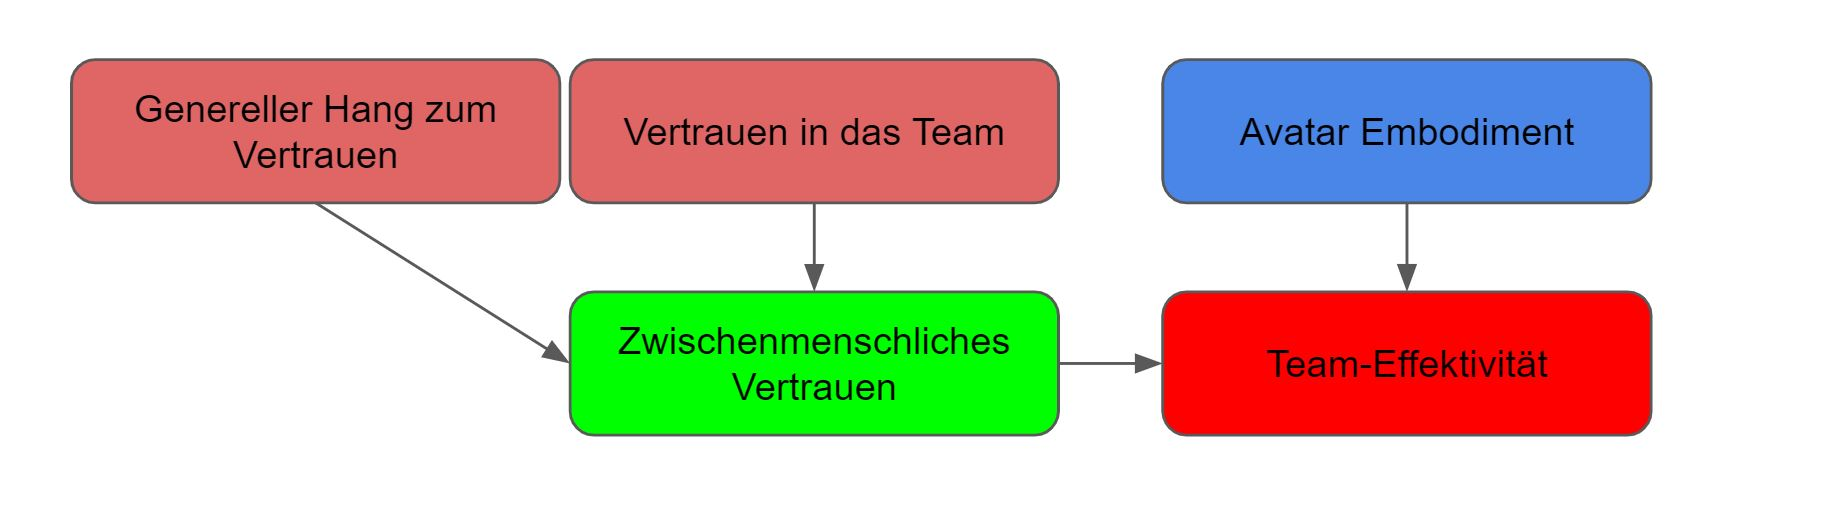
\includegraphics[width=\textwidth]{Abbildungen/Framework.JPG}\\
			\caption[Abbildung 1]{Das Framework}
			\label{Framework}
		\end{footnotesize}
	\end{figure}

Grundlage für das Framework \autoref{Framework} sind verschiedene wissenschaftlich basierten Quellen, die sich mit der \ac{vr} sowie zwischenmenschlichem Vertrauen befassen. Diese beiden Teilbereiche wurden kombiniert und soll versuchen, die Team-Effektivität anhand variierendem zwischenmenschlichen Vertrauen und verschiedenen Avatar-Verkörperungen zu messen.

Wie an dem Framework zu erkennen ist, wird davon ausgegangen, dass die beiden Faktoren \flqq Generelles Vertrauen\frqq sowie \flqq Vertrauen in das Team\frqq das \flqq Zwischenmenschliche Vertrauen\frqq zu gleichen Teilen beeinflussen. 

Weiterhin hat die Kombination des \flqq Avatar-Embodiment\frqq sowie des \flqq Zwischenmenschlichem Vertrauen\frqq ebenfalls einen Einfluss zu gleichen Teilen.

Da dies jedoch das erste mal ist, dass dieses Framework theoretisch Aufgestellt wurde, kann es sein, dass die verschiedenen Faktoren nicht zu gleichen oder auch gar keinen Einfluss auf die Team-Effektivität haben.

	\newpage
	\section{Grundlagen}
		\subsection{Virtual Reality}
		\subsubsection{Wozu brauchen wir Virtual Reality?}
			\subsubsection{Virtuelle 3D-Welten}
Virtual-Reality ist eine Realität, die durch den Computer, geschriebenen Computercode sowie erstellte 3D-Welten, abgebildet und zum Leben erweckt wird. Dabei Spielt der Nutzer, der in diese Eintaucht, das Immersive Erlebnis dessen sowie die Interaktivität in dieser, eine Zentrale Rolle. \citep[p.6-12]{sherman2018understanding}
	Seit vielen Jahren sind \ac{sve}'s Forschungsgrundlage der Virtuellen Realität. Siehe \citep{shuffler2011there} \citep{steed1999leadership} und \citep{de2011level} \\
	\ac{sve}'s bieten die Möglichkeit, Geographisch getrennte Benutzer in einem Virtuellem Raum zu verbinden. Diese stellen Nutzern der Virtuellen Realität die Möglichkeit bereit zu kommunizieren und zu interagieren. \citep[p. 1-3]{pettifer1999designing} Eine gute Übersicht der Anwendungsgebiete eines \ac{sve} wurde von Richard Waters dargestellt. Siehe dafür \citep{waters1997rise}.
	Zum Erfüllen dieser Studie wurde ein \ac{sve} entwickelt, welches den Nutzern ein \grqq Hand- und Kopf getrackten Avatar\grqq oder ein \grqq Hand-, Kopf und Inverskinematisch-simuliertem Torsos getrackten Avatar\grqq Avatar, je nach Anwendungsfall, zur Verfügung stellt. Innerhalb des \ac{sve} können sich die Nutzer frei bewegen, andere Avatare Wahrnehme und mit diesen interagieren.
	
			\subsubsection{Presence in Virtual Reality}
			
			Dank heutiger Technologien ist es uns möglich zu jeder Zeit mit Personen an verschiedenen Orten zu kommunizieren. Dadurch ist Kommunikation nicht mehr nur auf die Personen in unserer unmittelbaren Umgebung beschränkt. 
			Diese Neuerung ermöglicht es, uns nicht mehr nur auf \grqq Soziale Interaktionen \glqq mit physischen Wesen zu beschränken, sondern erweitert diese auch auf Repräsentationen geschaffen aus Pixeln, E-Mails, Film oder dem Telefon. Je nachdem wie Stark diese Repräsentation von uns Wahrgenommen wird, schafft Sie es, kraftvolle Emotionen in uns auszulösen.\citep[p. 4-6]{biocca2002defining}\\
			Nur wenn eine gewisse Präsenz dieser Repräsentation besteht, können Teambuildingmaßnahmen erfolgreich sein. Somit definiert das Vorhandensein des Gefühls von Präsenz den Grundbaustein für alle weiteren Schritte.\\
			Der Begriff \grqq Präsenz \glqq ist nicht genau definiert. Am ehesten trifft die Beschreibung zu, dass Presence das subjektive empfinden ist, an einem anderen Platz zu sein, obwohl man physikalisch eigentlich woanders ist. \citep[p. 1]{witmer1998measuring}\\
			Wenn eine Person eine andere Person in einer \ac{ivr} als Präsent wahrnimmt, werden die Wahrnehmenden, vestibulären, propriozeptiven und autonomen Nervensysteme in einen Zustand gebracht, der einem realen Zustand gleicht. Obwohl die betroffene Person weiß, dass Sie sich nicht in einer realen Lebenssituation befindet, wird diese dazu neigen, sich so zu verhalten, als ob diese in einer ist und Ähnliche Gedanken und Gefühle haben. \citep{slater2003note}

Diesbezüglich kann Präsenz als eine Art von Illusion angesehen werden, da die erzeugte Stimuli in der \ac{vr}, wie in der Realen Welt auch auf unsere Receptoren projeziert werden.

Somit lässt sich Präsenz in der \ac{vr} in 4 verschiedene teilbereiche gliedern.

\begin{itemize}
	\item{Die Illusion, sich in einem stabilen räumlichen Ort zu befinden} : Alle Stimuli zur räumlichen Wahrnehmung - wie zum Beispiel keine Restriktionen des \ac{fov} \footnote{Sichtfeld}, keine Kabel am \ac{hdm} - sollten sich möglichst wie in der realen Welt verhalten. \citep[p.47]{jerald2015vr}
	\item{Die Illusion der Selbstverkörperung} : Beschreibt das Gefühl einen Körper in der virtuellen Umgebung zu haben. Studien fanden heraus, dass durch einen virtuellen Körper die Präsenz in der \ac{vr} stark steigt. \citep[p.756]{botvinick1998rubber} Der virtuelle Körper muss nicht unserem eigentlichem ähnlich sehen. \citep[p.7]{maxwell1960psycho}
	\item{Die Illusion von körperlichen Interaktionen} : Beschreibt beispielsweise das vorhanden sein von Audio Feedback oder die Vibration des Controllers. Diese Kleinigkeiten tragen eine große Menge dazu bei, Präsenz in der \ac{vr} zu steigern. \citep[p.48]{jerald2015vr}
	\item{Die Illusion von sozialer Kommunikation} Sozialer-Realismus kann vom Physischen-Realismus abgetrennt werden. Social-Präsenz beschreibt das Gefühl, wirklich mit jemandem in einem \ac{sve} zu kommunizieren. Sei es verbal oder durch Körpersprache. Je mehr Nutzer der virtuellen Welt sich so verhalten, als ob diese real wäre, desto mehr steigt auch die Social-Präsenz. \citep[p.49]{jerald2015vr} \citep[p.12]{guadagno2007virtual}
\end{itemize}

\begin{figure}[H]
		\begin{footnotesize}
		\centering
			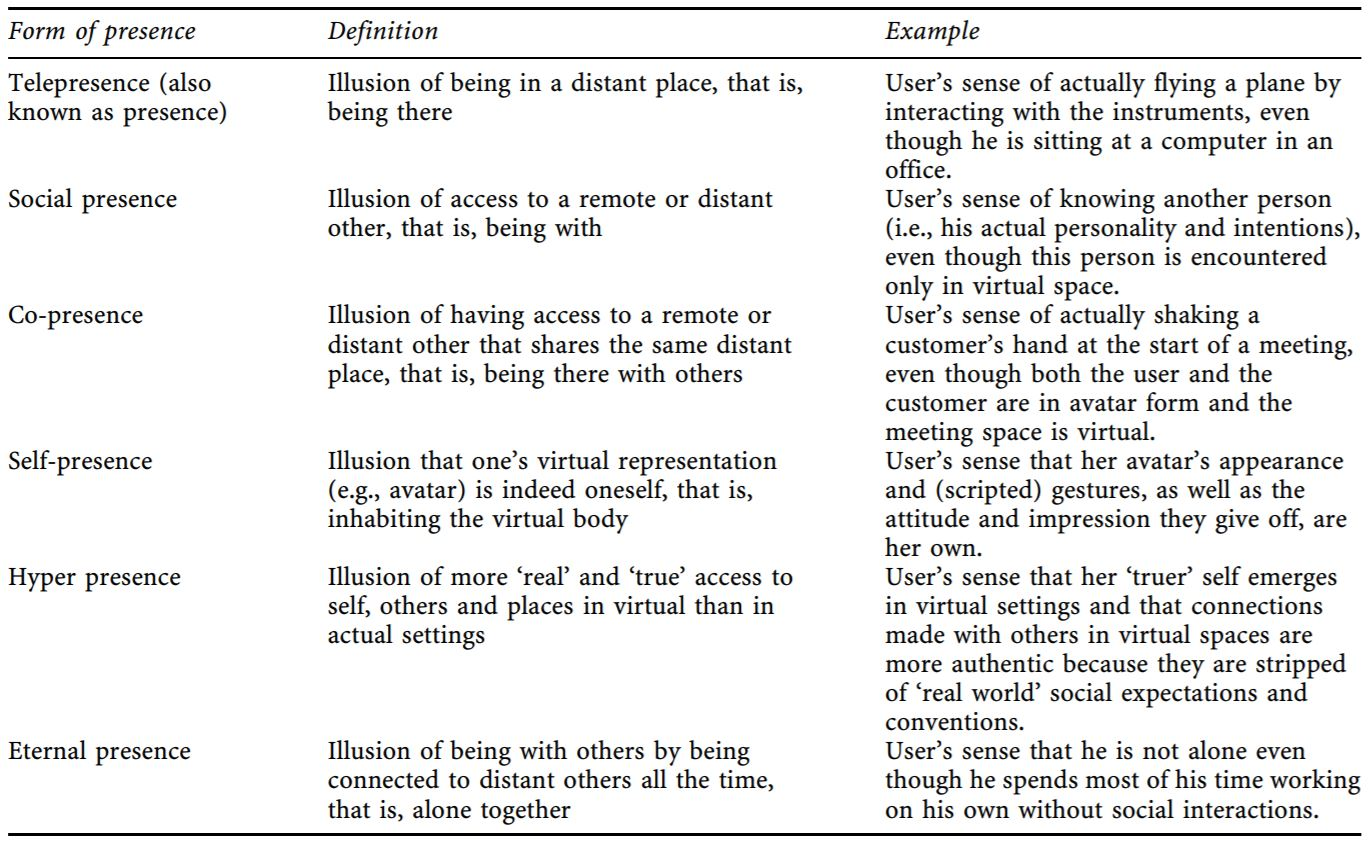
\includegraphics[scale= 0.4]{Abbildungen/forms_presence.JPG}
			\caption[Abbildung 1]{Forms of Presence}
			\textit{Die Verschiedenen Formen von Presence laut U.  Schultze \citep{schultze2010embodiment} }
			\label{vertical_horizontal}
		\end{footnotesize}
	\end{figure}


			Präsenz ist ein Konstrukt aus Immersion und dem Nutzer. Immersion kann ein Gefühl von Präsenz erschaffen, muss es aber nicht zwangsläufig. Je Immersiver ein System ist, desto höher ist das Potential dieses Systems, dass der Nutzer ein Gefühl von Präsenz entwickelt.
			
Lombard unterscheidet 6-Arten von Präsenz. Diese unterteilen sich in :
	\begin{itemize}
		\item \textbf{Sozialer Reichtum} : Das Medium wird als empfindlich oder persönlich wahrgenommen, wenn es zur Interaktion mit anderen Menschen verwendet wird.
		\item \textbf{Der Realismus} : Beschreibt die Wahrnehmung oder/und den Realismus der Präsenz und bis zu welchem Grad dieser als "Real" dargestellt werden kann.
		\item \textbf{Das Transportmedium} : Dies beschreibt das Gefühl "Du bist da", "Es ist da", oder/und "Wir sind Zusammen".
		\item \textbf{Die Immersion} : Beschreibt, wie Flächendeckend die Sinne des Benutzers angesprochen werden.
		\item \textbf{Der soziale Akteur innerhalb des Mediums} : Beschreibt die Reaktion auf eine Repräsentation einer Person durch ein Medium, auch wenn diese Irrational begründet ist.
		\item \textbf{Das Medium als sozialer Akteur} : Beschreibt die Situation wo der Akteur ( z.B. Computer ) selber als ein soziales Wesen wahrgenommen wird.					
				\citep{lombard1997heart}
			\end{itemize}
			Diese Arbeit richtet sich Hauptsächlich an die Präsenz als Transportmedium und das \grqq Das Medium als sozialer Akteur \glqq, da Personen die sich in der \ac{ivr} befinden, sich häufig als \grqq Präsent \glqq bezeichnen. Wenn Personen sich zusammen in einer \ac{ivr} befinden,  wird die Bezeichnung \grqq Co-Presence bzw. Social Presence \glqq genutzt. \citep{schuemie2001research}\\
			Es wird davon ausgegangen, dass eine \ac{sve}'s mehr Soziale Präsenz erwecken kann als Beispielsweise eine E-Mail. Dies sei damit begründet, dass \ac{sve} die Eigenschaften und Interaktionen des anderen besser darstellen und einfangen kann. Desto mehr Eigenschaften einer Person dargestellt werden können, desto höher ist der wahrgenommene Realitätsgrad des anderen. \citep[p. 5-8]{biocca2002defining}
			
Somit reicht das gesamte Kontinuum der Präsenz von der räumlichen Komponente bis hin starken psychiologischen Beteiligungen. Dies macht es möglich, auch auf die affektiven und kognitives Zustände von Personen aufzudecken. Höhere wahrgenommene Präsenz führt dazu, dass die Person sich mehr mit der \ac{vr} engagieren kann, was zu Handlungen führt, die als verbunden und voneinander abhängig wahrgenommen werden. \citep{biocca2001criteria}

\subsubsection{Vorbedingungen für Präsenz}
Um Präsenz in einer \ac{vr} zu erreichen, wird eine Schnittstelle zur Interaktion zwischen den Sinnen und der Außenwelt benötigt. Dies kann ein \ac{hdm} sein, welches ein computergeneriertes Bild erzeugt, durch das die virtuelle Welt wahrgenommen werden kann. Darüberhinaus muss das \ac{hdm} in der Lage sein, den Kopf des Benutzers frei im Raum zu Verfolgen und die gewonnenen Positionsdaten auf die \ac{vr} abzubilden. Weiterhin werden Controller benötigt, durch deren Einsatz es ebenfalls möglich ist, auch die Handbewegungen der realen Personen zu Verfolgen und diese in der \ac{vr} darzustellen. Das \ac{hdm}, die Controller, eventelle zusätzliche Körpertracker, Kopfhörer, eventuell Wahrgenommener Geruch etc. definieren, zu welchem Ausmaß Sinnesmodalität in der \ac{vr} generiert werden können. Der Grad der Immersion hängt somit direkt mit der Anzahl der angesprochenen Sinnesmodalitäten zusammen. Je mehr Sinnesmodalitäten auf einmal angesprochen werden, desto mehr ist der Wahrnehmungsapparat in der Lage, die virtuelle Umgebung auf die reale Welt abzubilden. \\
Somit lässt sich sagen, dass die Voraussetzungen für Präsenz in der \ac{vr} die Korrelation zwischen den Sinneseindrücken, der Propriozeption und dem Grad der wahrgenommenen Realität der Illusion, sich in einem stabilen räumlichen Ort zu befinden, darstellt. Sind diese Voraussetzungen gegeben, kann der Nutzer einen plausiblen Vergleich zwischen realen sensorischen und virtuellen, durch Illusion erzeugten Daten, aufstellen. \citep{slater2009we}

\subsubsection{Selbst-Avatar und Nicht-Selbst-Avatare}

\ac{hdm}'s beeinflussen das Sichtfelds des Nutzers so stark, dass diese Ihre eigenen Körper nichtmehr sehen können. Um diesem Nachteil entgegenzuwirken, kann einem Nutzer ein virtueller Körper zur Verfügung gestellt werden. Diesen Körper nennt man Selbst-Avatar.
Es ist schwierig einen Selbst-Avatar hoher Qualität zu simulieren. Dazu wäre im idealfall das Verfolgen und Animieren mehrerer Körperteil unabdingbar. Ist der Selbst-Avatar schlecht animiert oder es entstehen während der Nutzung Trackingfehler die der Nutzer erkennt, kann sehr leicht zu einem \ac{bip} kommen, bei dem die gesamte Illusion der \ac{vr} in sich zusammenbricht. 
Dies ist auch der Grund, weshalb relativ wenige \ac{vr}-Anwendungen den menschlichen Körper als Avatare darstellen.
Sind jedoch genügend Körperteile getracked und animiert, muss der Avatar nicht unverwechselbar menschlich aussehen um Self-Präsenz zu vermitteln, selbst grobe Avatar-Darstellungen schaffen es, ausreichende Informationen über die Glaubwürdigkeit eines menschlichen Körpers zu Vermitteln.\citep{lok2003effects}
Biocca forschte schon Umfangreich über den Einfluss von Self-Avataren auf den Nutzer in einer \ac{vr} \citep[421-427]{construal2014connected} So beispielsweise, wie sich die Interaktion mit der Welt verändert, wie sich soziale Interaktionen verändern und wie Aufgaben wahrgenommen und erledigt werden. \citep{benford1995user} \citep{bowers1996talk}
Studien gehen davon aus, dass ein menschlicher Körper als Avatar die Self-Präsenz stark erhöht.
Forschungen haben ebenfalls untersucht, wann und unter welchen Umständen ein Nutzer der \ac{vr} einen Selbst-Avatar als eigenen Körper wahrnimmt. 

Yee und Bailenson fanden heraus, dass der Proteus-Effekt den Nutzer so beeinflusst, dass sozialen Interaktionen des Nutzers denen der sozialen Identifikation seines Avatars ähneln. \citep{ratan2015leveling} Diese Abbildung der Verhaltensweisen des Nutzers lässt sich auch auf den Gruppenkontext beobachten. Der Nutzer wird sich in einer Gruppe so Verhalten, wie die Gruppenkonformität es vorgibt.
Dieser Effekt kommt nicht nur bei unverwechselbar Menschenähnlichen Avataren vor. \citep{lok2003effects} 
Solche identitätsbezogenen Avatar-induzierten Effekte, können somit die Kognitiven-Einstellunggen und Verhaltensweisen anderer Personen gegenüber beeinflussen.

Dodds fand heraus, dass ein Selbst-Avatar eine wichtiger Faktor zur Kommunikation in einem \ac{sve} ist. \citep[1-11]{dodds2011talk}

Connected to My Avatar:
Effects of Avatar Embodiments on User Cognitions, Behaviors,
and Self Construal 

421
https://sci-hub.do/10.1007/978-3-319-07632-4 


\subsubsection{Vertrauen in Avatare}
			
George, Eiband, Hufnagel und Hussman verglichen, ob sich mehr Vertrauen, entweder zwischen einem Menschenähnlichem oder einem Roboter-Avatar, aufbaut. Dazu schufen Sie ein Szenario, in dem Probanten mittels eines \ac{hdm}, ein Social-Dilemma-Scenario  \footnote{Situationen, in denen - die rationale Verfolgung von Eigeninteressen zu einer kollektiven Katastrophe führen kann, erlebten. Sie fanden keinen signifikanten unterschied in der Vertrauenswürdigkeit zwischen Menschenähnlichen und Roboter-Avataren. Jedoch wurde ein größeres Gefühl von Zusammenheit festgestellt, wenn mit einem Menschenähnlichem Avatar interagiert wurde. \citep{kerr1983motivation}}
Sie erwähnten ebenfalls in Ihrer Studie, dass hohe Grafik und Realistisches Verhalten durch beispielsweise Mikrogestikulationen, soziale Interaktionen sowie die Co-Präsenz fördern. \citep{george2018trusting}

Bente, Rüggenberg und Krämer führten 2004 eine Studie zur Sozialen Präsenz von Avataren in einem \ac{sve} durch. Dieses \ac{sve} war ähnlich einer Videokonferenz aufgebaut. Es waren keine \ac{hdm}'s vorhanden und die Teilnehmer sahen sich nicht. Sie verglichen dazu verschiedene Kommunikationarten, wie zum Beispiel Face-to-Face, Chat und Avatarbasierte kommunikationen untereinander, um Unterschiede in der Social-Presence sowie dem zwischenmenschlichen Vertrauen festzustellen.
Es wurde festgestellt, dass wenig Kognitives-Vertrauen zu Avataren aufgebaut werden konnte, während Face-to-Face, Telefon und Chatkommunikationen besser abschnitten. Weiterhin wurde weniger Affektives-Vertrauen als bei der Telefon oder Face-to-Face kommunikation aufgebaut.
Bente, Rüggenberg und Krämer gehen davon aus, dass dies mit der Neuheit der Technologie zusammenhängt. \citep[p.54-59]{bente2004social}
			
\subsubsection{Repräsentationen von Avataren}

Das Menschliche Gehirn ist in der Lage, computergenerierte Darstellungen in \flqq Lebend und Nicht-Lebend \frqq zu kategorisieren. Einige Forschungen gehen davon aus, dass das menschliche Gehirn semantische Unterschiede im zusammenhang mit der Social-Presence feststellen kann. So kann eine menschenähnliche Form als biologisch oder nicht-Lebend erkannt werden. 

	\begin{figure}[H]
		\begin{footnotesize}
		\centering
			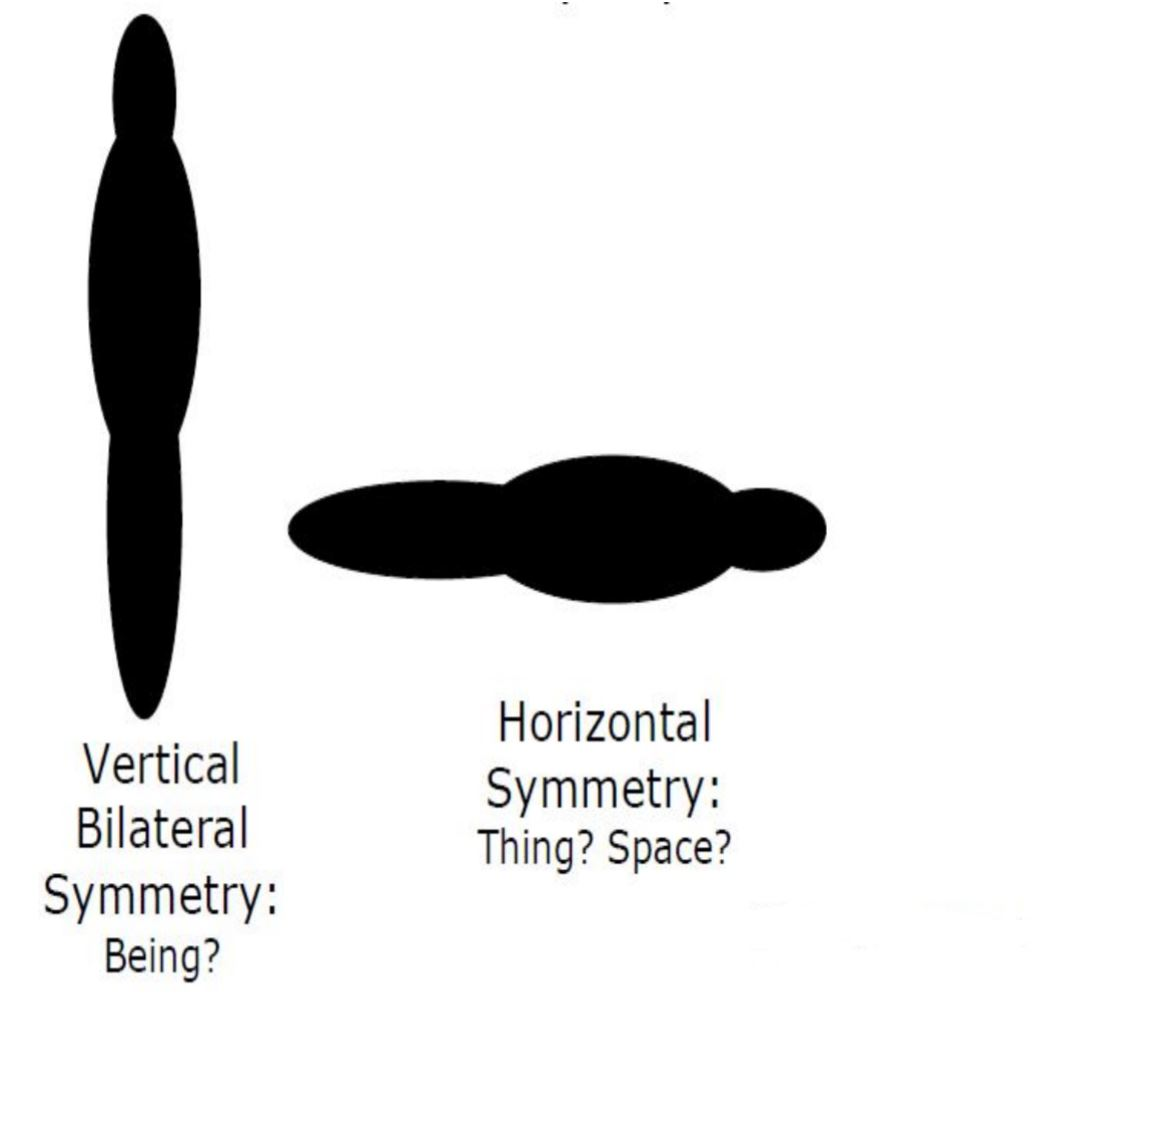
\includegraphics[scale= 0.4]{Abbildungen/Symmetry.JPG}
			\caption[Abbildung 1]{Social presence response to vertical and
horizontal beings}
			\textit{Menschen interpretieren symmetrische Formen um eine vertikale Achse eher als \flqq Menschlich\frqq als Formen um die horizontale Achse. \citep{biocca2002defining} }
			\label{vertical_horizontal}
		\end{footnotesize}
	\end{figure}

In \autoref{vertical_horizontal} ist zu erkennen, dass eine menschenähnliche vertikale, bilateral Symmetrische Repräsentation mehr Co-Präsenz erweckt als die horizontale bilateral Symmetrische Repräsentation. \citep[p.546-551]{thornhill1998relative}
Bilateral-Vertikale Symmetrie wird vom Menschen mit der körperlichen Gesundheit eines Menschens in Verbindung gebracht. Sogar Weibchen verschiedener Spezies neigen dazu, Partner mit einem höheren Grad an bilateraler Symmetrie auszuwählen. \citep]p. 659–669]{rhodes1998facial} \citep{biocca2002defining} \citep[p.233–242]{grammer1994human} \ \\

\begin{figure}[H]
		\begin{footnotesize}
		\centering
			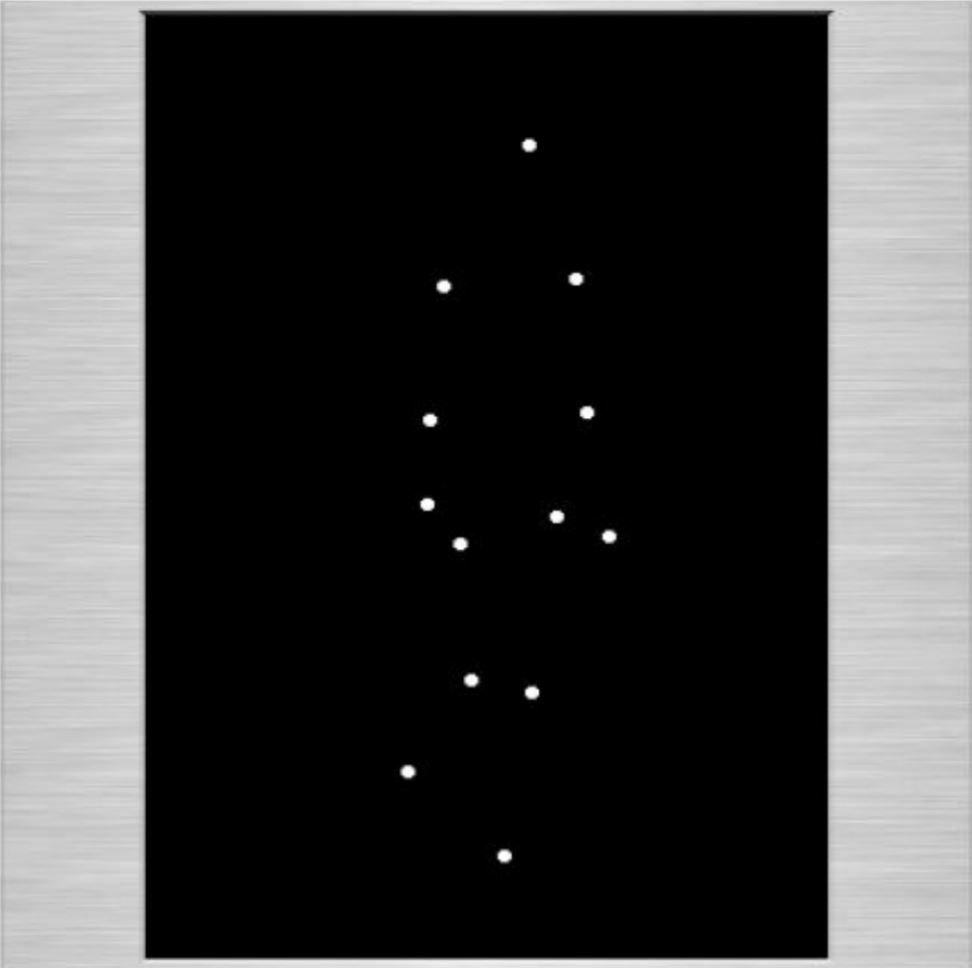
\includegraphics[scale= 0.5]{Abbildungen/moving_dots.JPG}
			\caption[Abbildung 1]{Social presence response to vertical and
horizontal beings}
			\textit{Stationäre punkte, bei denen der Mensch eine lebendige Bewegung ausmachen kann, wenn diese Anfangen sich zu bewegen. Es ist sogar möglich einen Menschen zu erkennen, dessen Art der Aktivität sowie den emotionalen Zustand. \citep{biocca2002defining} \citep[p.76-89]{johansson1975visual}}

			\label{moving_dots}
		\end{footnotesize}
	\end{figure}

Auch sich bewegende Punkte können als intelligentes Wesen wahrgenommen werden. Johannson \citep[p.76-89]{johansson1975visual} führte eine Studie durch, in der die Teilnehmer dreizehn \autoref{moving_dots} sich bewegende Punkte sahen und sofort die Darstellung einer menschlichen Bewegung erkennen konnten. Als die Punkte stationär waren, ist es den Teilnehmern der Studie nicht möglich gewesen diese Punkte als menschliche Repräsentation zu erkennen. Wenige Punkte reichen aus um Informationen zu erzeugen, die Aufschluss über die Aktivität, das Geschlecht, die Bewegung, den emotionalen Zustand oder die Anzahl der Personen zu geben.


			\paragraph{Computer-Mediated Communication}
			Nichtverbale Kommunikation -Beispielsweise nur via Text- erzeugt keinen Mehrwert an Vertrauen, Zusammenhalt und erzielt keine ausreichend gute Kommunikation. \citep[p.81]{haslam2003social}
			
			Allgemeine Kommunikation findet nicht nur mit Wörtern, sondern über Körpersprache wie Gestiken oder andere nonverbale Verhaltensmuster, statt. Durch \ac{sve}'s ist es nun möglich diese reine Text oder Bildbasierte Kommunikation durch Gestikulationen eines Avatars zu ersetzen. Durch diesen zusätzlichen visuellen Aspekt ist eine ganz neue Art und Weise der Kommunikation möglich, die nun gemessen werden kann.
			
			\subsubsection{Presence und Teambuilding}
			
			\subsection{Nonverbale Kommunikation}

Nonverbale Kommunikation kann Gesichtsausdrücke, Blicke, Bewegungen etc. umfassen. Kendon definiert im \flqq Kendon Kontinuum\frqq mit dem Begriff \flqq Gestik\frqq unwissende Gestiken (natürliche Körpersprache) bis hin zu \frqq Zeichen\flqq, welche alle durch Gestikulation erzeugten Zeichen ( z.B.O.K. Handzeichen ), beinhaltet. \citep[37]{mcneill1992hand} 
Im Rahmen dieser Arbeit, ist mit Gestikulation jedoch die gesamte Körperbewegung des Avatars gemeint.

Mehrabian zeigt in seiner Forschung, dass nonverbale Kommunikation zu 55\% dafür verantwortlich ist, ob ein gesprochenes Wort Positiv, Negativ oder Neutral interpretiert wird. Die Tonhöhe trägt zu 38\% und das eigentlich gesprochene Wort mit 7\% zur Interpretation bei. \citep[43]{mehrabian1971silent}

\textbf{Auf dieser Grundlage lässt sich davon ausgehen, dass, wenn interpersonelle Vertrauensbildung mitunter auf der Grundlage von Kommunikation stattfindet, der sprachliche Anteil mit 45\% einen Signifikanten Anteil zur Vertrauensbildung beiträgt und in einer Interpretation der Ergebnisse berücksichtigt werden muss.} \textbf{WAS MACHE ICH MIT DIESEM FOUND? IST INTERESSANT UND AUCH WICHTIG FÜR DIE VERTRAUENSFORSCHUNG IN RICHTUNG NONVERBALER KOMMUNIKATION}

%http://mcneilllab.uchicago.edu/pdfs/dmcn_vietri_sul_mare.pdf

%https://sci-hub.ren/https://doi.org/10.1371/journal.pone.0025759 SEITE 2
	
	\newpage
		\subsection{Teambuilding}		
		
		\subsubsection{Wozu brauchen wir Teambuilding?}
		\paragraph{Definition}
	Ein Team wird definiert als eine kleine Gruppe von Menschen mit gleichartigen Fähigkeiten, welche sich in gleicher Weise für das gleiche Ziel und gleiche Arbeitsweisen einsetzen und diese verfolgen.\citep[p. 2]{zenun2007effects}
	\\
Das Verhalten von Personen, die in einem Team arbeiten, lässt sich in \glqq Teamwork \grqq und \glqq Taskwork \grqq unterteilen. \citep[p. 541-542]{rousseau2006teamwork} Taskwork beschreibt, was für eine Aufgabe ein Team erledigt, sowie, wie die Ausführung von Kernkompetenzen in einem bestimmten Bereich aussieht. Teamwork beschreibt, wie ein Team gemeinsam eine Aufgabe erledigt. Dies beinhaltet, wie sich interaktive sowie voneinander abhängige Verhaltensprozesse zwischen Mitgliedern des Teams auswirken um eine Aufgabe zu erledigen. \citep[p. 357]{marks2001temporally} 
		
	Erfolgreichen Teambuildingmaßnahmen können die Effektivität eines Virtuellen Teams steigern und dazu führen, dass Personen sich mehr mit der Gruppe identifizieren. \citep{kaiser2000student}
		
	Teambuilding zielt dabei darauf ab, die Haltung oder Einstellung der Personen innerhalb eines Teams zu verbessern um das gesamte Team zu stärken, während Teamtraining drauf abzielt, spezielle Fähigkeiten einzelner Personen zu fördern um das gesamte Team zu stärken. \citep[p. 367-369]{shuffler2011there}\
		
	Die wirtschaftliche Leistung von Unternehmen hängt häufig stark von der Arbeitseffizienz gut funktionierender Teams ab. Teambuilding kann somit helfen, die wirtschaftliche Leistung zu verbessern, indem Mitgliedern eines Teams weniger Fehler durch bessere Entscheidungen erzeugen. \citep[p. 1-6]{biech2007pfeiffer} 
	
Virtuelle Teams entstehen zu lassen, stellt nicht die herausforderung dar. Die eigentliche Herausforderung ergibt sich aus den Unterschiedlichen Kulturen, Entfernungen und Zeitzonen, die ein Virtuelles Team mitbringt. Ist es nun jedoch möglich Vertrauen in das virtuelle Team zu bringen, kann der Nachteil auch zum Vorteil werden. Es wird mehr Kulturelle Diversität gefordert, wodurch neue, kreative Sichtweisen gefördert werden. Durch diese Faktoren ist es letztendlich möglich Innovativer zu Arbeiten und zu denken. \citep{dyer1995team} \citep[p.405-416]{milliken1996searching}

	\subsection{Einflussfaktoren im Teambuilding}

%Emotional Contagion with Artificial Others. Effects
%of Culture, Physical Appearance, and Nonverbal Behavior
%on the Perception of Positive/Negative Affect in Avatars 	

412

%https://sci-hub.do/10.1007/978-3-319-07632-4
	
	
An Investigation into Gender Role Conformity in an Online Social
Networking Environment.......................................... 322

Gesture and facial expression
Gesture is an important part of conversation and ranges from almost sub-conscious accompaniment to speech to complete and well formed sign languages for the deaf. Support for gesture implies that we need to consider what kinds of 'limbs' are present. Facial expression also plays a key role in human interaction as the most powerful external representation of emotion, either conscious or sub-conscious. Facial expression seems strongly related to gesture. However, the granularity of detail involved is much finer and the technical problems inherent in its capture and representation correspondingly more difficult. A crude, but possibly effective approach, might be to texture map video onto an appropriate facial surface of a body image (e.g. the "Talking Heads" at the Media Lab [2]). Another approach involves capturing expression information from the human face using an array of sensors on the skin, modelling it and reproducing it on the body image (e.g. the work of ATR where they explicitly track the movement of a user's face and combine it with models of facial muscles and skin [6] and also the work of Thalmann [10] and Quéau [7]).
This discussion of gesture and facial expression relates to a further issue, that of voluntary versus involuntary expression. Real bodies provide us with the ability to consciously express ourselves as a supplement or alternative to other forms of communication. Virtual bodies can support this by providing an appropriate set of limbs and 'strings' with which to manipulate them. The more flexible the limbs; the richer the gestural language. However, we suspect that users may find ways of gesturing with even very simple limbs. On the other hand, involuntary expression (i.e. that over which users have little control) is also important (looks of shock, anger, fear etc.). However, support for this is technically much harder as it requires automatic capture of sufficiently rich data about the user. This is the real problem we are up against with the facial expression issue - how to capture involuntary expressions.

%https://dl.acm.org/doi/fullHtml/10.1145/223904.223935?casa_token=B8tEKM39OVQAAAAA:VNilOxaXG3_2Bw-bEClS10xyOXLBxB8ymyo4B-d1kUoAmCgWC1MDdVKSptRADsBaGw19nzE15dwIWQ


	Z.b. Aussehen, Kulturen, etc.	
	
	\subsubsection{Teambuilding in virtuellen Teams}
%	https://sci-hub.tw/https://doi.org/10.1108/13527590110395621

Seit einigen Jahren wurde die Wichtigkeit von effektiven Teambuildingmaßnahmen in der strategischen Organisationsentwicklung erkannt. Dabei spielt der Wandel hin zu einer globalen, auf Wissen basierten Wirtschaft eine zentrale Rolle. \citep{belbin2011management} \citep[p.7]{katzenbach2015wisdom}
Wirtschaftlicher Erfolg korreliert direkt mit der Fähigkeit eines Unternehmens Teams organisieren, strukturieren und managen zu können. \citep{pasmore1993designing}
Der Erfolg eines virtuelle Teams ist somit als Nebenprodukt der oranisatorischen Fähigkeiten eines Unternehmens zu verstehen. \citep[Chapter.5]{kling1994social}
	Gerade für virtuelle Teams ist die Anfangsphase des Teambuilding von entscheidender Bedeutung. Mitglieder von virtuellen Teams haben im Gegensatz zu traditionell geformten Teams weniger Möglichkeiten sich zu sehen, zu interagieren oder Konflikte zu lösen. 
Respekt und gegenseitiges Verständnis sind die Grundbausteine um Kreativität und Innovation innerhalb eines Teams zu fördern, die Effizienz eines Teams ist eine direkte Konsequenz daraus.
Vertrauensaufbau im Team nimmt eine wichtige Rolle in virtuellen Teams ein, denn im Gegensatz zu traditionellen geformten Teams haben Teammitglieder eines virtuellen Team keine Möglichkeit durch geselliges Beisammensein oder durch physischen Kontakt Bindungen aufzubauen um das gegenseitige Vertrauen zu stärken.\citep{TrustAndTheVirtualOrganisation}  \\
Vertrauen in einem Team zu fördern ist somit eine Notwendigkeit um Wachstum und Erfolg des Teams zu bestimmen. 
\citep{glacel1997teamwork} \\
Eine idiale Teambuilding Situation ist daher in virtuellen Teams nicht möglich. (Cianni andWnuck, 1997) ( Hier einfügen oder doch als eigenen Satz stehenlassen? )
Virtuelle Teams werden trotz der Konsequenzen der räumlichen und zeitlichen Trennung gebildet, ohne die vorherigen Beschriebenen Vorteile in kauf zu nehmen. Die Optimale Situation wäre es, in einem schon bestehendem Team eine virtuelle Komponente hinzuzufügen um auf die Vorteile von schon vorhandenen sozialen Bindungen zugreifen zu können. \citep[p.36-37]{holton2001building}
Es sollte sichergestellt werden, dass virtuelle Teams während ihres Bestehens bestmöglichst in ihrem Aufbau von Vertrauen und sozialen Beziehungen unterstützt werden, um den Erfolg des Teams möglichst zu gewährleisten.

	\subsubsection{Aktuelle Teambuildingmaßnahmen in virtuellen Teams}


\textbf{Überleitung zu Virtual Reality finden}


	\subsubsection{Kooperativ vs Kompetitive}
	
		\subsubsection{Effektivität von Teambuildingmaßnahmen}
		
	\textit{\textbf{Team efficiency: Team efficiency refers to the team’s ability to interact with each other in a way that supports the team’s goals while also taking external factors into account. Hence team efficiency is concerned with different teamwork processes. It is connected to team performance/ effectiveness which relates to the team’s ability to achieve certain results (Salas,Sims und Burke, 2005). EINFÜGEN HIER?}}
	
	In einem Team sind viele verschiedene Personen mit unterschiedlichen Verhaltensweisen und Einstellungen involviert. Dies führt zu einer Steigerung der Qualität der Ideen und Entscheidungen sowie der gesamten Teamleistung.
	Die Kommunikation untereinander wird gefördert, da die einzelnen Teammitglieder gegenseitig ihre Aufgaben kennen und dadurch eher bereit sind sich untereinander zu helfen.
	Geteiltes wissen bedeutet größeren Lerneffekt, was mit einem besseren Verständnis über das Wissen des anderen einhergeht. Somit können auch individuelle Stärken gefördert, und schwächen durch andere Teammitglieder kompensiert werden.
	Ein Team bringt ein Gefühl von Sicherheit mit sich, was zu einer erhöhten Risikobereitschaft führt. Dies erhöht die Kreativität der eingebrachten Ideen können entstehen und Teammitglieder an der Möglichkeit größere Risiken einzugehen wachsen. \citep[p. 2-4]{biech2007pfeiffer}
	
	Es gibt keinen einheitlichen Standard um die Performance eines Teams zu messen. Es wird davon ausgegangen, dass die Effektivität in Gruppen anhand der von der Gruppe produzierten Ergebnissen (Quantität, Qualität, Geschwindigkeit, Kundenzufriedenheit) gemessen werden kann. Eine Gruppe hat Einfluss auf die Produktivität der einzelnen Mitglieder, von diesem Effekt profitiert die gesamte Gruppe und trägt somit zur Verbesserung der Gesamteffektivität bei. \citep[p.309]{guzzo1996teams}
	
	Training im Team kann die gesamte Performance eines Teams steigern. Das Training im Team scheint am effektivsten, wenn mehrere Charakteristika des Teamworks auf einmal angesprochen werden. Diese sollten auch experimentelle Aktivitäten beinhalten um aktiv zu lernen und zu üben. \citep[19]{mcewan2017effectiveness}
	
	
		\subsubsection{Teambuilding Komponenten}
	\textit{\textbf{HIER NOCHMAL KURZ ERKLÄREN WOZU DIE TEILBEREICHE EIGENTLICH DA}}
	Teambuilding kann in 10 verschiedene Teilbereiche unterteilt werden. Siehe \autoref{ten_characteristics}
	\begin{figure}[H]
		\begin{footnotesize}
			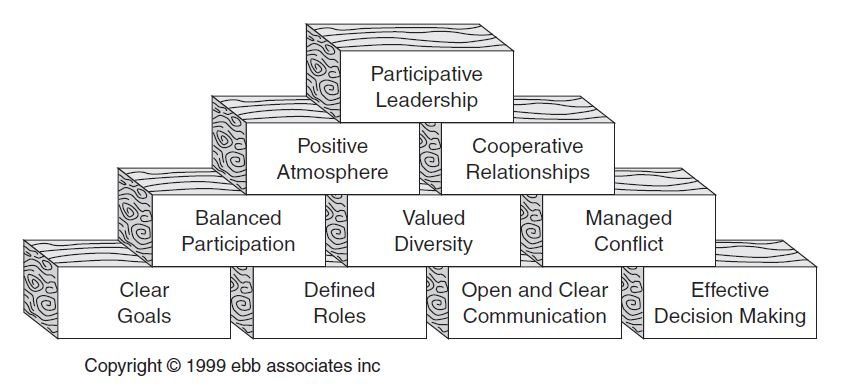
\includegraphics[width=\textwidth]{Abbildungen/Ten_Characteristics.JPG}
			\caption[Abbildung 1]{Ten Characteristics of a High Performance Team \citep[p. 27]{biech2007pfeiffer}}
			\label{ten_characteristics}
		\end{footnotesize}
	\end{figure}
	Die einzelnen Teilbereiche bauen aufeinander auf. Der untere Teilbereich mit den Komponenten \textit{Clear Goals"}, \textit{Defined Roles}, \textit{Open and Clear Communication} sowie \textit{Effective Decision Making} sind die Basis des gesamten Models. Diese Komponenten sollten am Anfang des Teambuildingprozesses definiert und immer als Basis der gesamten Teamarbeit gesehen werden.\\
	Der Teilbereich mit den Komponenten \textit{Balanced Participation}, \textit{Valued Diversity} und \textit{Managed Conflict} baut auf diese auf.\\
	\textit{Positive Atmosphere} und \textit{Cooperative Relationships} ist der dritte Teilbereich. In diesem geht es hauptsächlich um die Zufriedenheit und die Bereicherung eines einzelnen in einem Team zu arbeiten. Jedoch ist dieser Bereich nicht mehr Ausschlaggebend um eine Aufgabe zu erledigen. Für viele Teammitglieder ist dieser Teilbereich jedoch wichtigste Ziel während der Teamarbeit.\\
	\textit{Participative Leadership} ist der einzige Bereich der aus dem Gesamtgebilde ohne Beeinflussung der anderen Komponenten entfernt werden kann. Dies sagt uns, dass ein Teamm auch ohne einen einzelnen Teamleiter existieren kann. Vgl. \citep[p. 13-16]{biech2007pfeiffer}\\
	Aufgrund der vielen Komponenten die ein Team erfüllen muss um effizient zu sein und ein Gestärktes Teamgefühl zu bilden, wird in dieser Ausarbeitung nur auf einen Teilbereich eingegangen.
	
	\paragraph{Positive Atmosphere}
	Wird der Aufbau von Vertrauen vernachlässigt, so bildet sich kein gut funktionierendes Team.
	\paragraph{Open and Clear Communication}
	\paragraph{Balanced Participation}
	\paragraph{Defined Roles}
	
		\subsubsection{Team-Colloboraton}
		\subsubsection{Virtual-Teambuilding}
		
		\paragraph{Allgemeines}
		Virtuelle Teams werden häufig gebildet um räumliche oder kurzzeitige Trennungen eines Teams zu umgehen. Dabei werden computergestützte Technologien verwendet. \citep[p. 1-2]{cascio2003leadership}
		
		Virtuellen Teams ist es möglich, dass räumlich getrennte Teammitglieder ihre Aufgaben, mittels computergestützter Kommunikation, im Team koordinieren können. \citep[p. 117-119]{peters2007identifying} \textbf{117,118,119 - Seitenzahl nicht sicher}
		
		Es kann effizient Länderübergreifend gearbeitet werden, was ein größeres Innovationspotential für Unternehmen zur folge hat.	
		Virtuelle Teams haben den Ruf teuer zu sein, die Ziele nicht verfolgen zu können, nie pünktlich und schwierig zu managen zu sein. \citep[p.243-244]{gassmann2003trends}
		
		Virtuelle Teams sind häufig gerade in der Anfangsphase sehr Ergebnisorientiert in der Art und Weise \textit{wie} kommuniziert wird. Dieses Defizit in der Sozialen Kommunikation untereinander kann die Schlüsselfaktoren eines Erfolgreichen Teams beeinträchtigen - Soziale und Emotionale Beziehungsbildung sowie den Aufbau von Vertrauen. \citep[p.378]{ren2007applying} \\
		Um die Wahrscheinlichkeit zu erhöhen, dass auch in der Anfangsphase des Teambuildings eine \glqq Soziale\grqq und keine \glqq Arbeitsnahe, Ergebnisorientierte\grqq Kommunikation stattfindet, wurde eine spielerische Umgebung geschaffen, in der sich das Team das erste mal kennenlernen kann. 
		
Virtuelle Teams werden in dieser Arbeit als temporär, divers und räumlich gerennt, beschrieben. Die Kommunikation untereinander nur durch das World-Wide-Web statt. Weiterhin impliziert die temporäre Eigenschaft der Definition, dass sich die Teammitglieder nicht kennen.
		
		\paragraph{Social Identity}
		Personen fühlen sich zu einer Vielzahl von Gruppen hingezogen. Das Soziale Identitätsgefühl hängt davon ab, ob ein generelles Gruppenverständnis besteht, eine Person sich der Gruppe zugehörig fühlt und ob man sich zu als Gruppe mit anderen Gruppen vergleicht. Gruppenzugehörigkeit ist ein wichtiger Bestandteil des Selbstverständnisses eines Individuums. \citep{sutantovicious}
		Ist gute Gruppenzugehörigkeit gegeben, stärkt dies die Gruppenproduktivität sowie die individuelle Leistungsfähigkeit. Weiterhin entstehen dadurch Effekte die zum besserem Zusammenhalt, mehr Vertrauen \citep{herbsleb2000distance}, besserer Kommunikation und Kooperation untereinander führen. \citep[p. 510]{olson2003psychological}
		
		
		\subsubsection{Vorteile/Nachteile von Teambuilding}
		
		\subsection{Trust}
Vertrauen in die \ac{vr} kann auf zwei weisen Betrachtet werden. Das Vertrauen in die Akzeptanz von \ac{vr} sowie das zwischenmenschliche Vertrauen, welches in der \ac{vr} zwischen 2 oder mehreren Personen gebildet werden kann.

Mangelndes Vertrauen in eine Technologie, kann Nutzer dran hindern, diese zu Nutzen. \citep{trustInVRTechnology}

Da diese Arbeit sich mit dem zwischenmenschlichem Vertrauen beschäftigt, wird das zwischenmenschlichem Vertrauen betrachtet.
		\subsubsection{Wozu brauchen wir Vertrauen im Allgemeinen?}
		Vertrauen ist ein Psychiologischen Konzept, dass jeden Menschen im täglichem Leben begleitet.
Vertrauen gilt als einer der Grundbausteine im Unternehmertum. Ohne Vertrauen in Ihr Team oder in Unterschiedliche Personen, fällt es schwer Risiken einzugehen. Ist Vertrauen vorhanden, wird man nicht mit der Angst konfrontiert, dass andere Personen einen ausnutzen könnten. \citep[p.1152]{breuer2016does}.
Vertrauen wird als ein bilaterales Konstrukt zwischen einer vertrauenden Person und einer zu vertrauenden Person definiert.
\citep[p.728-729]{mayer1995integrative}
Betrachtet man Vertrauen auf Teamebene, setzen sich die Vertrauenden Personen sowie die zu Vertrauenden Personen aus mehreren Teammitgliedern zusammen.
 Mayer definiert Vertrauen als :"a willingness of a party to be vulnerable to the actions of another party based on the expectation that the other will perform a particular action important to the trustor, irrespective of the ability to monitor or control that party" \citep[p.712]{mayer1995integrative} \\

		\subsubsection{Zwischenmenschliches Vertrauen}
		https://sci-hub.tw/https://doi.org/10.1177/1046496408323569
Während Vertrauen in Technologie sich mit der Akzeptanz dieser Beschäftigt, beschäftigt sich zwischenmenschliches Vertrauen mit dem Vertrauen zwischen zwei oder mehreren Personen. \citep{mcknight2011trust}

Viele Forschungen, die sich mit dem Thema Vertrauen beschäftigen, gehen von aus, dass zwischenmenschliches Vertrauen aus einem zweidimensionalem Konstrukt besteht. \citep{johnson2005cognitive} \citep{cook1980new}

Cook und Wall beschreiben diese Zwei Dimensionen als  \begin{itemize}
\item{ “faith in the trustworthy intentions of others”, sowie}
\item{“confidence in the ability of others, yielding ascriptions of capability and reliability”.}
\end{itemize}


\paragraph{Affektives- und Kognitives Vertrauen}
Diese beiden Dimensionen bestätige McAllister ebenfalls in seinen Forschungen. Er definierte die beiden Punkte als Kognitives Vertrauen und Affektives Vertrauen.
Affektives Vertrauen ergibt sich somit aus zwischenmenschlichen emotionalen Verbindungen und gegenseitiger Fürsorge, während individuelles kognitives Vertrauen auf der Überzeugung in die Fähigkeiten oder in die Zuverlässigkeit eines anderen basiert. \citep{mcallister1995affect} \\

\textbf{ES GIBT NOCH MEHR VERGLEICHE, SIEHE DAZU QUELLE UNTEN}
\textbf{HIER EINEN VERGLEICH ZWISCHEN COGNITIVE TRUST UND AFFECTIVE TRUST AUFSTELLEN. AUCH BEIM FRAGEBOGEN BEACHTEN! ERKLÄRUNG GEBEN WARUM GENAU DEN VON MC ALLISTER 1995 GENOMMEN WURDE.}
http://citeseerx.ist.psu.edu/viewdoc/download?doi=10.1.1.496.9380&rep=rep1&type=pdf

Vertrauen im Team wird meinst jedoch nur eindimensional gemessen, obwohl es ein zweidimensionales Konstrukt ist.
Polzer, Crisp, Jarvenpaa und Kim haben Beispielsweise eine Forschung über räumlich getrennte Teams und deren Vertrauensbildung durchgeführt, eine eindimensionale Affektive Vertrauensmessung. \citep[p.682]{polzer2006extending}
Prichard und Ashleigh haben 2007 ebenfalls mit einer eindimensionalen Kognitiven Vertrauensmessung herausgefunden, dass Teambuilding Teamvertrauen stärkt. \citep[p.704]{prichard2007effects}
Dirks hat 1999 zwar die Multidimensionale Komponente aufgegriffen, jedoch stand für seine Versuchsdurchführung nur ein 10-Minütiges Zeitfenster zur Verfügung. In diesen 10-Minuten kann die Affektive-Komponente nicht gebildet bzw. gemessen werden. \citep[p.445]{mayer1995integrative} Daher wird seine Forschung ebenfalls nur als eindimensional betrachtet.
Mehrdimensionale, zuverlässige, Vertrauensforschung ist nur mittels Langzeitstudien möglich, \textbf{ IST DAS SO?}denn Kognitives- und Affektives-Vertrauen eine Zeitliche Komponente benötigt. \citep{jones1998experience} \\

Laut Forschungen von McKnight kann ein starkes Vertrauen auch in frühen Teambuildingphasen entstehen. Glauben Teammitglieder beispielsweise in frühen Teambuildingphasen, dass der Teambuildingprozess mit Strukturierungen und Regelungen durchwachsen ist, ergibt sich dadurch ein höheres kognitives Vertrauen und es folgt ein höheres Gesamtvertrauen in das Team.
\citep[p.478-479]{mcknight1998initial} \\

Daraus lässt sich schließen, dass, wenn Personen ein hohes Grundvertrauen haben, auch ein höheres Kognitives Vertrauen in frühen Phasen des Teambuildings besitzen. \\

Grundvertrauen setzt sich dabei aus der individuellen Eigenschaft des Hangs zum Vertrauen einer einzelnen Person, sowie die Grundstimmung gegenüber Personen im Allgemeinen, zusammen. \citep{couch1996assessment} \\

McKnight \citep[p.6]{mcknight2011trust} erwähnt in seiner Forschung, dass der \glqq generelle Hang zum Vertrauen\grqq die tendenz wiederspiegelt, anderen zu Vertrauen. Der Generelle Hang zum Vertrauen ist nicht Situationsabhängig, sondern Stellt eine längerfristige Konstante dar.

\textit{Hypothese H1} : \textbf{Probanten mit einem hohen General-Trust-Score erzielen auch einen hohen Kognitiven-Trust-Score.}
\\
\subsubsection{Vertrauen ins Team}

In vielen Forschungen wird behauptet, dass Vertrauen einen positiven Effekt auf die Teamperformance hat. \citep{mcallister1995affect} \citep{mayer1995integrative} \citep{dirks2002trust}
Kognitives Vertrauen lässt sich nur sehr schwer aufrechterhalten. So könnte es sein, dass ein Team einen hohen Kognitiven Vertrauenswert aufweist, dann jedoch einen Rückschlag bei einer Aufgabenerledigung erzielt. Dies hat eine Verringerung des Kognitiven Vertrauen des Teams zur folge. \citep[p.29-31]{mcallister1995affect}
Im Vergleich wird das affektive Vertrauen im Team bei solchen Situationen nicht verringert. Um eine Verringerung des affektiven Vertrauens zu verursachen, benötigt es eine längerfristige emotionale Kriese innerhalb des Teams. Somit stellt sich herraus, dass das affektive Vertrauen eine längerfristige, stärkere Bindung schafft, als das kognitive Vertrauen.  \citep[p.29-31]{mcallister1995affect} \\

\textit{Hypothese H3} : \textbf{Ein hoher Kognitiver-Trust-Score wirkt sich positiv auf die Team-Effektivität aus.}\\

\textit{Hypothese H5} : \textbf{Teams, mit einem generell hohem Hang zum Vertrauen erzielen auch eine hohere Team-Effektivität.}

		\subsubsection{Cognitive Trust}
		
		\subsubsection{Affective-Trust}
		
	\newpage
	\section{Versuchshypothesen}

Folgende Hypothesen wurden aufgestellt :
\begin{itemize}
	\item{H1 : Probanten mit einem hohen General-Trust-Score erzielen auch einen hohen Cognitiven-Trust-Score.}
	\item{H2 : Ein Torso, Head und Hand getrackter Avatar hat einen positiven Einfluss auf den Cognitiven-Trust-Score.}
	\item{H3 : Ein hoher Cognitiver-Trust-Score wirkt sich positiv auf die Team-Effektivität aus.}
	\item{H4 : Ein Torso, Head und Hand getrackter Avatar hat einen positiven Einfluss auf die Team-Effektivität.}
	\item{H5 : Teams, mit einem generell hohem Hang zum Vertrauen erzielen auch eine hohere Team-Effektivität.}
\end{itemize}

\textbf{NEU}

\begin{itemize}
	\item{H1 : Probanten mit einem hohen General-Trust-Score erzielen auch einen hohen Cognitiven-Trust-Score.}
	\item{H2 : Probanten, die einen Torso, Head und Hand getrackter Avatar nutzen erzielen einen höheren Cognitiven-Trust-Score.}
	\item{H3 : Ein hoher Cognitiver-Trust-Score wirkt sich positiv auf die Team-Effektivität aus.}
	\item{H4 : Ein Torso, Head und Hand getrackter Avatar hat einen positiven Einfluss auf die Team-Effektivität.}
	\item{H5 : Teams, mit einem generell hohem Hang zum Vertrauen erzielen auch eine hohere Team-Effektivität.}
\end{itemize}


Diese wurden in einer Grafik Veranschaulicht um einen besseren Gesamtüberblick zu erhalten.

\begin{figure}[H]
		\begin{footnotesize}
			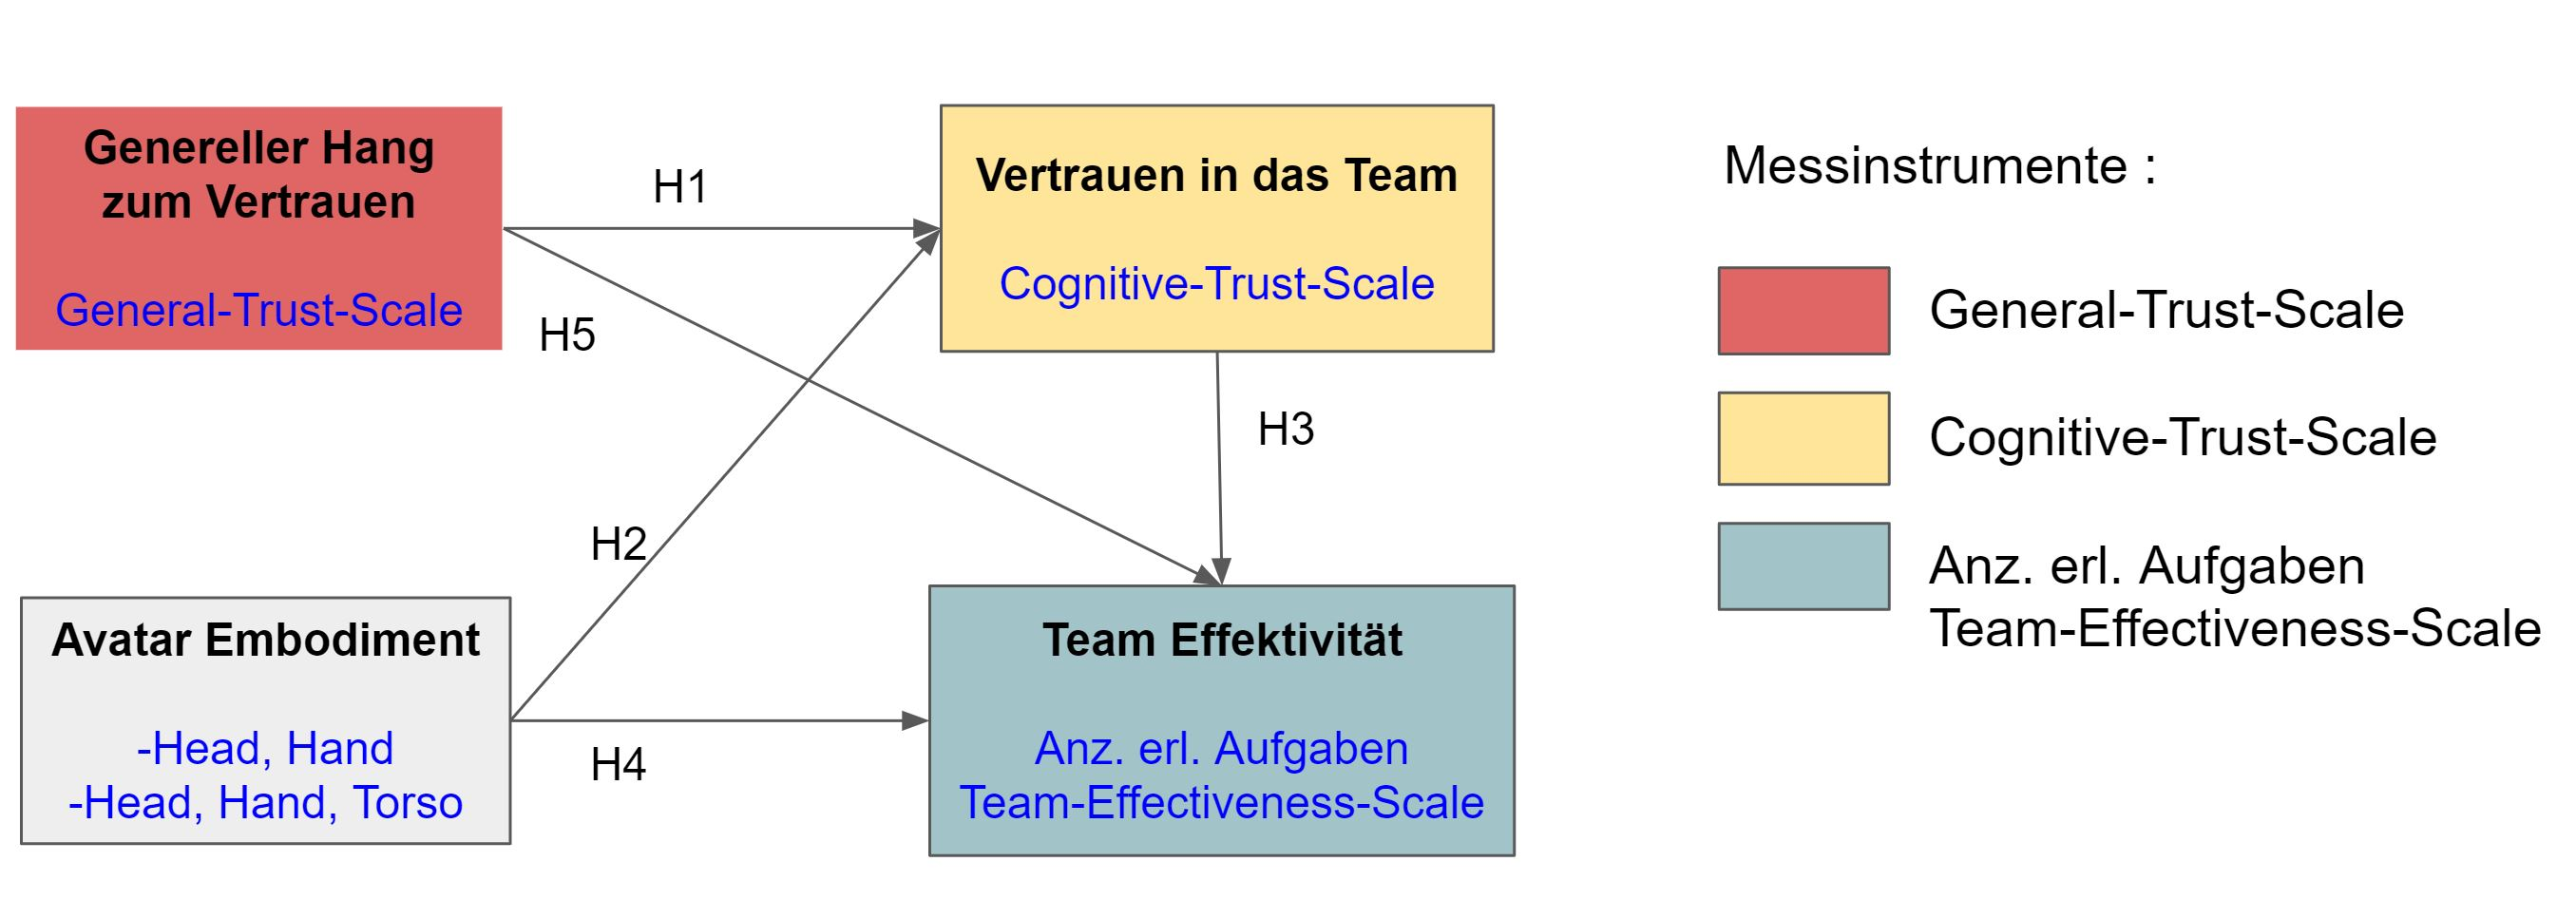
\includegraphics[width=\textwidth]{Abbildungen/Versuchshypothesen.JPG}\\
			\caption{Versuchshypothesen}
			\label{Versuchshypothesen}
		\end{footnotesize}
	\end{figure}	

		
	\section{Vorgehensweise}
		\subsection{Verwendete Technik}
			\subsubsection{Verwendete Hardware}
Um an dem Experiment Teilnehmen zu können, benötigten die Probanten ein im vollem Umfang funktionierendes HTC-Vive, HTC-Vive2 oder ein Oculus-Rift S \ac{hmd} mit funktionsfähigen Controllern sowie einen Leistungsstarken \ac{vr}-Fähigen PC. Der Spectator, der das Experiment Remote steuern und verwaltet, benötigt einen Leistungsstarken PC auf dem die Anwendung ausführbar ist.

			\subsubsection{Verwendete Software}
Das \ac{sve} wurde mit Unity 2019.4.3f1 und der HD-Render-Pipeline programmiert. Um die Echtzeitkommunikation zwischen den einzelnen Clients zu gewährleisten, wurde das multiplayer Framework \flqq Normcore\frqq \footnote{www.Normcore.io} genutzt.
Normcore unterstützt Network-Physics, automatische Realtime-Synchronisation, Voice-Chat, XR-Compitabilität sowie persistente multiplayer Räume.
		\subsection{Fragebogenentwicklung}
	
\textbf{USE THIS https://repository.upenn.edu/cgi/viewcontent.cgi?article=1068&context=od_theses_msod}
Um die Erfahrungen und Eindrücke der Teilnehmenden Probanten zu Quantifizieren, wurden einige standartisierte Fragebögen verwendet.
	
\begin{itemize}
\item{NASA-TLX} Der NASA-TLX misst die subjektiv wahrgenommene Arbeitsbelastung sowie Effektivität der Probanten innerhalb des \ac{sve}.
\item{Igroup Presence Questionnaire(IPQ)} Der IPQ dient zu Messung des Präsenzgefühls in einer virtuellen Umgebung. Dabei misst der IPQ, inwieweit sich der Nutzer in der virtuellen Umgebung fühlt, inwieweit der Nutzer seine Aufmerksamkeit der virtuellen Umgebung schenkt und wie Real die virtuelle Umgebung dem Nutzer erschien.
\end{itemize}
		Hier dran Beispiel nehmen:
		
		%https://d1wqtxts1xzle7.cloudfront.net/30602859/Presence_202004_20-_20Valencia.pdf?1361179740=&response-content-disposition=inline%3B+filename%3DOn_the_importance_of_reliable_real_time.pdf&Expires=1600808306&Signature=PFz5w5T5Gm4ikI5rIBhqVy~LMmhEofYpGS1x2oQCR39owjNnPEW28~Hjl8oE6k3hNT4A9I1ekCpSu9JLim6ro8TF8zAxuxuDmzfjr8Y8RF864oG71-xhGSlyLJ5iklLURCTQJciuJPc2A-Avq633G2LZHcQmIHQAm0Tfwrw5vokvWxco5DYMQXK8W9KXPue9OR0gK4xvhKKdWg4DTUdoy1TTdHRvcaBWLYI2960-ijiH6Ox2Rl8B2xxuWQfpvsdS~Vkz7k7A1F5LpVV8-w2Dn5WimnycBIp7UCodkjAeUdT~--KiD4~bdo8w4vEb6fm2xQMMw6NBWuTIqSNjSbjzlg__&Key-Pair-Id=APKAJLOHF5GGSLRBV4ZA#page=54
		\subsection{Zielgruppe}
		Die Voraussetzung um an dem Versuch Teilzunehmen, ist es, ein \ac{HDM}, zwei Controller sowie ein Computer mit Internetzugang zu besitzen. Der gesamte Versuch ist als ein "Into the Wild" Versuch aufgebaut, welches bedeutet, dass die genaue Zielgruppe nicht genau definiert werden kann. Die einzigen Ristriktion sind die vorher beschriebenen Konditionen. 
		
		\subsection{Untersuchungsmethode}
			\subsection{Qualitative vs Quantitative Untersuchung}
			\subsubsection{A/B Testing}
			\subsubsection{Teilnehmerfindung}
Da das gesamte Experiment als Into-the-Wild Experiment aufgebaut wurde, wurde in verschiedenen Foren ( z.B. VRForum.de, Computerbase.de, Hardwareluxx.de, etc. ) durch eine Suchanfrage, in Form eines extra dafür angelegten Threads, Teilnehmer gesucht. Weiterhin wurden Teilnehmer durch verschiede Facebookgruppen mit einem Bezug zu \ac{vr}, sowie durch zufällige Whatsapp-Chatgruppen mit 50+ Mitgliedern, akquiriert. Da das gesamte Experiment, sowie die Versuchsanleitung auf deutscher Sprache erstellt wurde, fand die Teilnehmerfindung nur im deutschsprachigem Raum statt.
			\subsubsection{Datenerhebungsmethoden}
			
			\paragraph{COMMUNICATION SCALE QUALITY}
			\textbf{After the experimental portion was completed, participants completed
another set of measures. First, participants completed the Communication Quality Scale
developed by González-Romá & Hernández (2014). This scale contains 5 items that assess
participants’ perceptions of their team’s communication quality, rated on a 1 to 5 scale. The full
measure is available in Appendix D}
\citep[p.1049]{gonzalez2014climate}

			\paragraph{Cognitive Trust Scale}
			\textbf{After each bomb was completed (successfully or not), participants filled out
a cognitive trust scale developed by Wildman et al. (2009) and based on the trust theory of
Lewicki, McAllister, & Bies (1998). This 8-item scale taps into participants’ trust attitudes and 
62
each item is rated on a 5-point scale from “not at all” to “very much so”. While this measure has
not yet been published, it has been validated in both lab and field samples and has shown utility
in prior teamwork research (Lazzara, 2013; Wildman, 2011). Appendix C contains the full scale}


			\paragraph{Generalized-Trust-Scale}
			
			\textbf{The propensity to trust measure developed by Couch, Adams, & Jones (1996) was
administered in order to gauge participants’ trusting dispositions. The Generalized Trust subscale
of this measure was utilized for this study. It contains 20 items (e.g. “I have few difficulties
trusting people”) and participants rated how strongly they agree with each statement on a 1
(strongly disagree) to 7 (strongly agree) scale. See Appendix B for the full scale. The full trust
inventory by Couch et al. (1996) also contains a Partner Trust subscale, but this was not relevant
to the study as it pertains to trust of one’s romantic partner.}
https://sci-hub.ren/10.1207/s15327752jpa6702_7
\citep{couch1996assessment}

			\paragraph{TEAM EFFECTIVENESS SCALE}
			\textbf{Next, participants completed a 5-item team effectiveness measure. This measure is
comprised of the Quality subscale from Gibson, Zellmer-Bruhn, and Schwab's (2003) Team
Outcome Effectiveness survey. Participants rated their agreement with each of the five items on
a 1 to 7 scale. The team effectiveness measure is available in Appendix E.
Last, participants indicated whether or not they were already familiar with their
teammate. If so, they were also asked to indicate approximately how many years they had known
their teammate, and how often they communicated with the teammate. Finally, teams were
prompted to write a few sentences about why they thought their team performed the way it did.
Effectiveness Measures}
			\citep[p.469]{gibson2003team}

				\paragraph{Fragenbogen}
Es wurden zwei Fragenbögen an die jeweiligen Studienteilnehmer verteilt. Der erste Fragenbogen wurde an die Probanten vor der eigentlichen Studie ausgefüllt. Ziel war es, die Einstellungen zu Teamarbeit sowie zu Interpersonellem Vertrauen der Personen vor der eigentlichen Untersuchung festzustellen. Der Zweite Fragebogen wurde nach der Untersuchung ausgefüllt, um die Effektivität der verschiedenen Konditionen der Untersuchung auf Erfolg oder Misserfolg untersuchen zu können.
				Es wurden nur vollständig Ausgefüllte Fragebögen zur Datenanalyse herangezogen. Konnte nicht ermittelt werden, welche Aussage angekreuzt wurde, wurde dieser ebenfalls nicht mit in die Datenanalyse aufgenommen. Eine Außnahme war dabei, falls ein Teilnehmer im Nachhinein nach die von Ihm gewünschte Antwort befragt werden konnte.
				\paragraph{Beobachtung}
				Durch die Beobachtung während des Experiments werden Kennzahlen zur Dauer des Versuchs zwischen den einzelnen Konditionen bestimmt. Anhand dieser kann im späterem Verlauf das  Teambuilding Potential sowie die subjektive Effektivität durch gesteigertem Swift-Trust analysiert werden.
				\paragraph{Induktive Quantitative Forschungsmethodik}
				Anhand der subjektiven Betrachtungsweise einzelner Personen des Themas "Vertrauen" wurde ein quantitatives Forschungsdesign gewählt anhand die Ergebnisse induktiv interpretiert und ausgewertet wurden.
		
\subsection{Unabhängige Variablen}
Als unabhängige Variablen wurden der \flqq IK-Avatar\frqq sowie der \flqq Non-IK-Avatar\frqq gewählt. Durch diese  unabhängigen Variablen wurde im weiterem Versuchsverlauf versucht den Einfluss auf die abhängigen Variablen zu bestimmen.
Insofern wird untersucht, wie der Einfluss von dem \flqq IK-Avatar\frqq sowie dem \flqq Non-IK-Avatar\frqq auf das Generelle-Vertrauen, das Vertrauen im Team sowie auf die Team-Effektivität ist.
			\subsubsection{Avatar embodiement}
				\paragraph{Head- and Handtracking}
				\paragraph{Head-,Hand and Inversekinematic-Torso}
	
\subsection{Abhängige Variablen}
			\subsubsection{Generelles Vertrauen}
			Wie in \textbf{Abbildung \ref{ten_characteristics}} beschrieben \textbf{ABBILDUNG 1 BESCHREIBEN, TRUST z.B. UND EINZELNE PUNKTE}, ist die Positive Atmosphere in einem Team einer der Maßgeblichen Faktoren die zur Leistungsfähigkeit und zum \textit{\glqq wir-gefühl\grqq} beitragen.
			Die Abhängige Variable Vertrauen ...	
			%\paragraph{Swift-Trust}
			%\subsubsection{Kommunikation}
			%\subsubsection{Team Zusammenhalt}
			%\subsubsection{Teambuilding Potential}
			\subsubsection{Vertrauen in das Team}
			\subsubsection{Team Effektivität}
			%\subsubsection{Andere Faktoren}
			
\subsection{Residuen}
			\subsubsection{Aufbau der Umgebung}
			\subsubsection{Farbe der Avatare}
			\subsection{Geschlecht}
			BSPW. Auf die Androgynität des Avatars eingehen
			\subsubsection{Sozialpsychologische Einflussfaktoren}
				\paragraph{Gamification} $~$ \\
				\paragraph{Aussehen} $~$ \\
				\paragraph{Sprache} $~$ \\	
				\paragraph{Bekanntheit}
Um die gegenseitige Bekanntheit der Probanten auszuschließen, wurde jedem Probanten zu beginn des Versuchs ein Zufälliger anonymer Name zugeordnet.
			
		\subsection{Beschreibung des Forschungsverlaufs}
		Insgesamt nahmen \textbf{ANZAHL DER TEILNEHMER} am Versuch teil.
Jeder Probant bekam einen zufälligen Zeitslot sowie ein anonymen Namen zugeordnet mit dem dieser an dem Versuch teilnahm. Gemäß des A/B-Testings wurden jeweils drei Personen in einem Zeitslot untergebracht um ein "Team" zu bilden. Diesem "Team" wurde entweder die Kondition "Head- und Handtracking" oder "Head-, Hand mit Inversekinematisch-simulierten-Torso" zugeordnet. Somit nahmen drei Probanten, an einem Versuch zur selben Zeit mit der selben Kondition, teil. Die Probanten wurden nicht Face-To-Face vorgestellt und sahen sich während des gesamten Versuchs nur als Repräsentation eines Avatars in der Virtuellen Umgebung. Der Zeitslot von 30 Minuten teilte sich auf in
		\begin{itemize}
			\item 5 Minuten Pre-Questionnaire
			\item 20 Minuten Versuchsdurchführung
			\item 15 Minuten Post-Questionnaire
		\end{itemize}
		Jeder Teilnehmer bekam zu beginn seines Zeitslots einen Pre-Questionnaire ausgehändigt, den dieser selbstständig ausfüllen sollte. In diesem wurden Fragen über die \flqq Person\frqq, über eventuelle \flqq Gesundheitliche Beschwerden \frqq sowie schon vorhandene \flqq \ac{vr}-Erfahrung\frqq, gestellt.
		Dieser wurde von \textbf{ANZAHL DER PERSONEN} Personen ausgefüllt. \textbf{Da nicht alle Fragebögen vollständig ausgefüllt wurden, konnten nur X Ergebnisse in die Analyse mit eingezogen werden.}
		Nachdem alle Probanten den Pre-Questionnaire ausgefüllt hatten, begann das Experiment. Dazu loggte sich das jeweilige Team in das \ac{sve} ein und spielten den Versuch durch.
		Während der Versuchsdurchführung wurden Notizen zum Verhalten der einzelnen Personen gemacht um herauszufinden, ob beispielsweise ein Probant die Teamleaderrolle übernahm, in welchem Maß interpersonelle Kommunikation stattfand oder wie die Teilnehmer auf die jeweiligen Avatare reagierten.
		Am Ende der Versuchsdurchführung, wurde ein Post-Questionnaire ausgeteilt. In diesem wurden Fragen über das \flqq Generelles Vertrauen\frqq, das \flqq Kognitive Vertrauen\frqq die \flqq Kommunikations-Qualität\frqq, die wahrgenommene \flqq Team-Effektivität\frqq, die \flqq Beanspruchung\frqq sowie die \flqq Präsenz\frqq, gestellt. Am Ende war es jeden Teilnehmer zusätzlich möglich ein Feedback zu geben. Der Post-Questionnaire wurde von \textbf{ANZAHL DER PERSONEN} Personen ausgefüllt. \textbf{Da nicht alle Fragebögen vollständig ausgefüllt wurden, konnten nur X Ergebnisse in die Analyse mit eingezogen werden.}
		
Die maximale Versuchsdauer nach Start der Anwendung betrug exakt 10 Minuten. Es konnten maximal 20 Runden absolviert werden, wobei jede Runde inkrementell schwieriger wurde, da jede 3. Runde jeweils 1 Symbol, in den Pool der zu erratenden Symbole, hinzukam. 


	\subsection{Allgemeiner Versuchsaufbau}

\begin{figure}[H]
		\begin{footnotesize}
			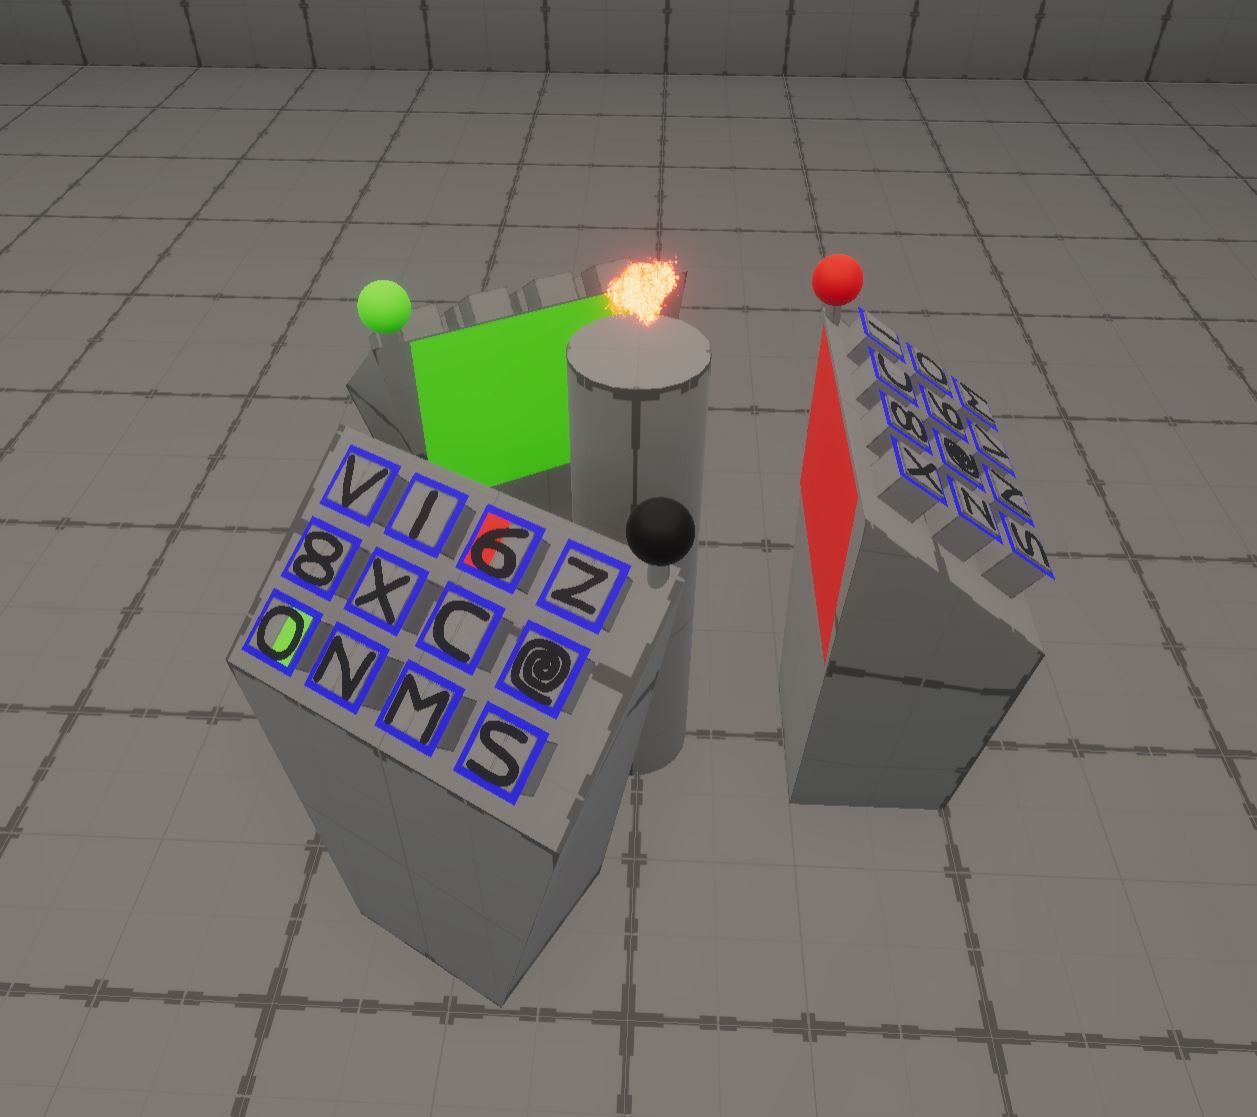
\includegraphics[width=\textwidth]{Abbildungen/Podeste.JPG}\\
			\caption[Abbildung 1]{}
			\label{Framework}
		\end{footnotesize}
	\end{figure}

Jeder Probant benötigte (neben einem funktionsfähigen Computer), um an dem Versuch teilnehmen zu können, entweder ein Oculus oder HTC-Vive \ac{hdm}, sowie zwei funktionsfähige Controller.

Dem Versuchsleiter war es während der gesamten Anwendung möglich, die 3 Probanten durch einen eigenen Client zu betreuen. Alle Probanten konnten durch Ihre Anwendung durch das integrierte Mikrofon im \ac{hdm} zu dem Versuchsleiter Sprechen und diesen hören. Während die Probanten sprachen, konnten die anderen zwei Probanten diese jedoch nicht hören. Die Sprachkommunikation eines Probanten war somit nur Richtung Versuchsleiter möglich. Dies dient zur Vermeidung von einigen Störvariablen und zum Erhalt der Integrität der Anonymität.
Während der Versuchsleiter sprach, konnten jedoch alle Probanten den Versuchsleiter hören. Dies diente dazu, eventuelle offene Fragen an alle Versuchsteilnehmer weiterzugeben und den Beginn sowie das Ende der Anwendung zu kommunizieren. Der Versuchsleiter gab jedoch während des gesamten Versuchs keine Hilfestellung.

In der Anwendung war es den Probanten möglich mittels der Tasten \flqq W A S und D\frqq ihre Position und mittels den Tasten \flqq Q\frqq und \flqq E\frqq ihre Höhe, in einem gewissen Bereich, zu ändern. Dies stellte sicher, dass alle Probanten ihre Avatargröße und Position individuell an ihre Körpergröße anpassen konnten.

Da es den Probanten nicht möglich sein sollte, auf die Symbole der anderen teilnehmenden Probanten zu schauen, wurde ab einer gewissen Grenze Links und Rechts des Podest der Probanten ein \flqq Fade-To-Black\frqq Mechanismus eingebaut. Kamen die Probanten mit dem Kopf ihres Avatars in diesen Bereich, sahen diese nur noch die Farbe Schwarz und mussten sich zurückbewegen.

Waren alle Probanten bereit, wurden diese vor ein für Sie eigenes Podest teleportiert und sahen einen Countdown zwischen den 3 Podesten herunter zählen. Dieser Countdown litt den baldigen beginn einer Runde ein.
Wurde eine Runde gestartet, wurde das Podest jedes Probanten eineindeutig durch die Farbe \flqq Schwarz, Rot oder Grün\frqq markiert. Die Probanten konnten Ihre und die Farbe des Spielers an einem Viereck sowie einer runden Kugel in der jeweils zugeteilten Farbe, an den jeweiligen Podesten, erkennen. Die Farbe der einzelnen Probanten änderte sich jede Runde.

	\subsection{Der Versuch}

Der Schwarz markierte Probant war mit dem Erklären in der jeweiligen Runde an der Reihe.
Auf dem jeweiligen Podest eines Probant befanden sich verschiedene Symbole. Diese Symbole waren für alle Probanten gleich, jedoch an unterschiedlichen Positionen. Der Schwarz markierte Probant hatte an den Symbolen noch entweder die Farbe \flqq Grün oder Rot\frqq oder \flqq Grün und Rot\frqq.
Der schwarz markierte Probant versuchte nun, mittels Hand und Armbewegung, den Rot und Grün markierten Probant die Symbole, die in der jeweiligen Spielerfarbe vor Ihm markiert waren, zu erklären.
Meinte ein Probant (Rot oder Grün), dem der schwarz markierte Probant ein Symbol erklärt hat, ein Symbol erkannt zu haben, loggte dieser das Symbol durch herunterdrücken des Knopfes an seinem Podest, mit dem jeweiligen erkanntem Symbol, ein. Der Schwarz markierte Probant musste nichts einloggen oder klicken, sondern nur durch Gestikulation erklären.
Hat ein Probant sich während des einloggens verklickt oder wollte seine Meinung zum erkanntem Symbol ändern, musste das Symbol vorher, durch erneutes klicken des Symbols vor ihm, ausgeloggt werden. Anschließend konnte es erneut eingeloggt werden.
Wurden alle Symbole vom roten und grünem Probant erkannt und eingeloggt, die der schwarz markierte Probant angezeigt hat, wurde dies durch eine grüne Kugel, für alle Sichtbar, erkennbar gemacht und die Runde endete. Erschien diese grüne Kugel nicht, war noch etwas falsch und der schwarz markierte Probant musste noch einmal versuchen die korrekten Symbole den jeweiligen Mitspielern aufzuzeigen.
In der nächsten Runde wurde ein anderer Probant eineindeutig mit Schwarz, Rot oder Grün markiert.
Mit steigender Anzahl an erfolgreich bestandenen Runden, müssen mehr Symbole erfolgreich erkannt werden.

Das Ziel war es nun, so viele Symbole wie möglich gemeinsam korrekt zu bearbeiten und dadurch in höhere Runden aufzusteigen.

	\subsection{Die Avatare}
Die Avatare im \ac{sve} wurden als \flqq IK-Avatar\frqq und \flqq Non-IK-Avatar\frqq implementiert.
Für beide Avatararten wurde die neutrale Farbe Schwarz gewählt. Die Probanten hatten keinen Einfluss auf die Farbwahl ihres eigenen Avatars. Dies dient dazu die Störvariable der eventuell vorhandenen Vorurteile des Mitspielers aufgrund der Farbe des Avatars, auszuschalten. Je nach Kondition \flqq IK-Avatar\frqq oder \flqq Non-IK-Avatar \frqq bekam jeder Probant das Selbe aussehen des Avatars zugeordnet. Der eigene Avatar ist nicht für die Mitspieler sichtbar. Zur besseren Interaktion mit den Knöpfen sowie zur höheren Immersion, wurde der eigene Avatar nicht sichtbar für den Probanten dargestellt. Jeder Probant, unabhängig der zugewiesenen Kondition sah somit nur eine Repräsentation von menschlich wirkenden Händen.

	\begin{figure}[H]
		\begin{footnotesize}
			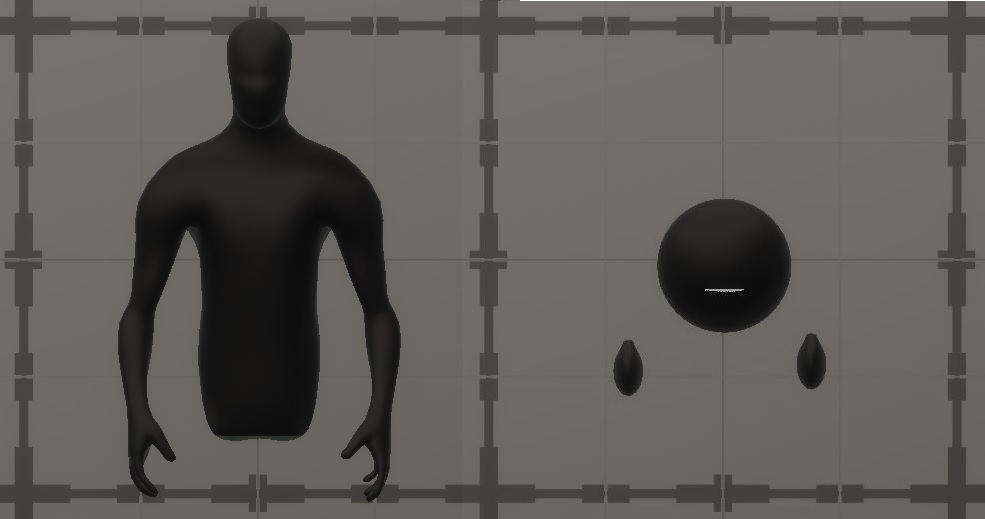
\includegraphics[width=\textwidth]{Abbildungen/Avatars.JPG}\\
			\caption[Abbildung 1]{Links: IK-Avatar, Rechts: Non-IK-Avatar}
			\label{Framework}
		\end{footnotesize}
	\end{figure}

		\paragraph{IK-Avatar}
Der Invers-Kinematisch getrackte Avatar hat ein Androgynes aussehen, um die Störvariable rund um Vorurteile aufgrund des Geschlechts der Probanten auszublenden. Der IK-Avatar besitzt keine Augen, Mund, Haare oder Beine. 
Um eine Möglichst realistische Bewegung zu erzielen, wurde die Handbewegung, die Unterarmbewegung, die Oberarmbewegung sowie die Kopf-und Brustrotation simuliert.

		\paragraph{Non-IK-Avatar}
Der Non-IK-Avatar besteht aus einem Kreis mit Mund sowie einer Repräsentation der Linken sowie der Rechten Hand. Er Besitzt keine Augen, Haare, Beine, Hals, Torso sowie Ober- und Unterarm. Der Mund dieses Avatars ist als unauffälliger Orientierungspunkt des Kopfes erhalten geblieben. Der Mund des Non-IK-Avatars bewegt sich jedoch nicht. 
	\newpage
	\section{Ergebnisse}
		\subsection{Validität und Reliabilität}
		Validität : Eventuell gibt es für die Probanten der Studie einen "Neuheitseffekt", weshalb unzureichend das Vertrauen analysiert werden kann. Der "Wow"-Effekt ist eventuell sehr groß. Weiterhin kann es sein, dass durch die Tatsache, dass einige Leute schon die VR Kennen, eine andere Einstellung zu dem Thema haben und deshalb nicht mehr ganz Valide antworten.
		Weshalb ist meine Forschung Valide? Weshalb ist sie reliabel?	
		\textit{BEISPIEL : Die Forschung ist valide, da immer dieselbe Waage verwendet wurde, die exakt nach europäischen Standards wiegt. Zudem wurde die Reliabilität der Waage während der Untersuchung täglich getestet, indem ein Kilogramm Blei darauf gelegt wurde. Jedes Mal zeigte die Waage dabei ein Kilo an.}
		\subsection {Gesammelte Daten}
	
		\subsection{Analyse}
	\newpage
	\section{Zusammenfassung}
	\newpage
	\section{Diskussion}
		\subsection{Diskussion der Ergebnisse}
		\subsection{Diskussion der eingesetzten Methoden}
		\subsection{Auswirkungen auf die Gegenwart}
		\subsection{Vorschläge für zukünftige Untersuchungen}
		Social Identity und Teambuilding - Ein Avatar ist anders.
	
	\newpage
	\appendix	
	\section*{Anhang}\markboth{Anhang}{Anhang}\addcontentsline{toc}{section}{Anhang}
	Den Anhang beginnen Sie auf einer neuen Seite und in einem neuen Abschnitt. Die Überschrift selbst wird nicht nummeriert.
	
	\begin{figure}[H]
		\begin{footnotesize}
			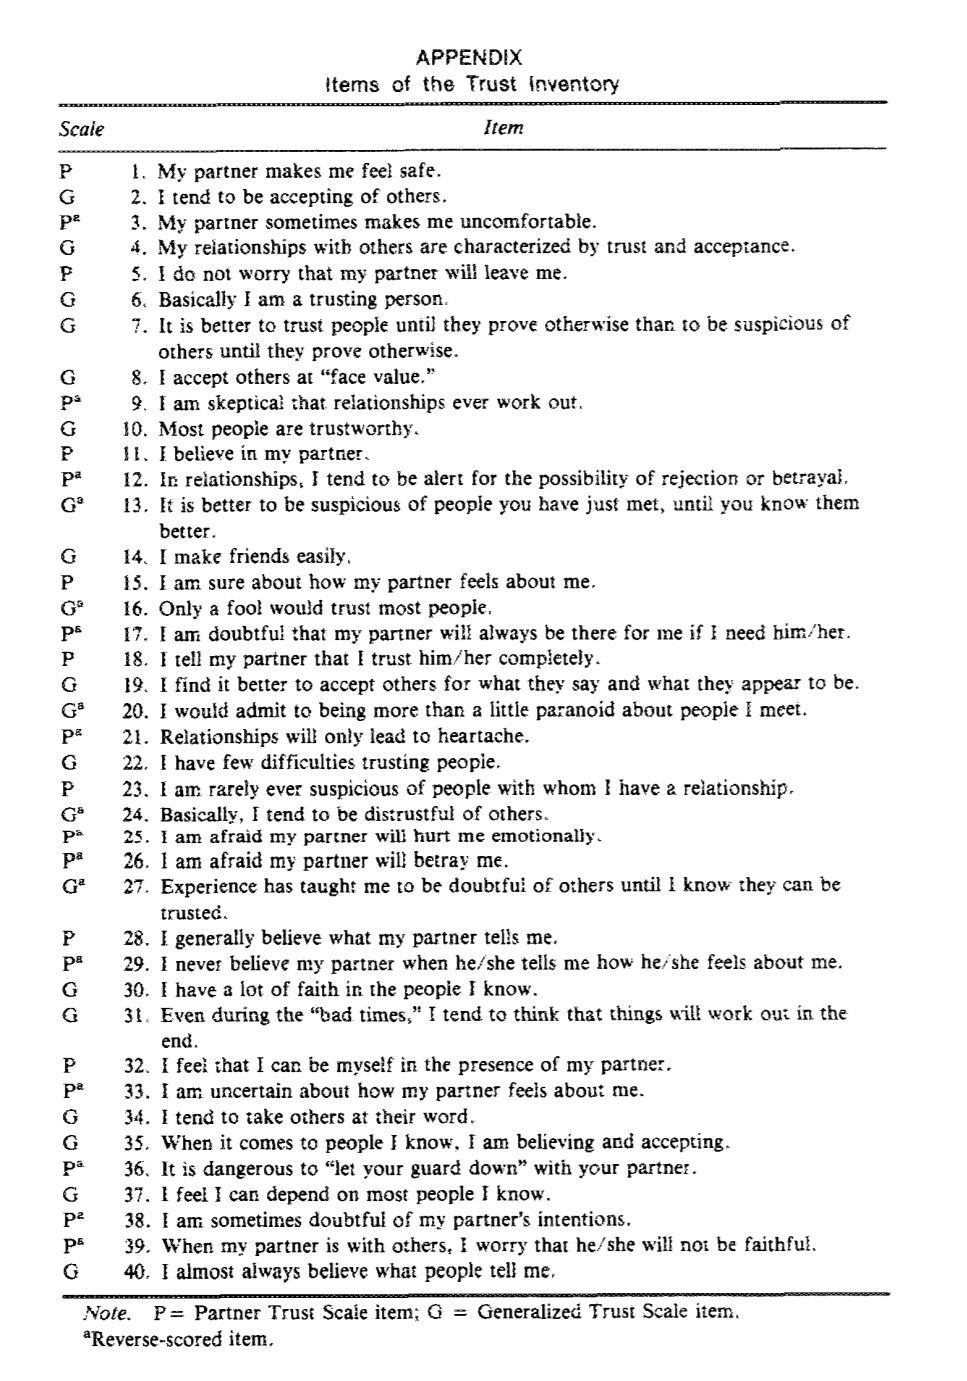
\includegraphics[width=\textwidth]{Abbildungen/CouchEtAl_1996_TrustScale}\\
			\caption[Abbildung 1]{Items of the Trust Inventory \citep[305-323]{couch1996assessment}}
			\label{Trust-Inventory}
		\end{footnotesize}
	\end{figure}
	
	\newpage

\bibliographystyle{dcu}
\bibliography{bibfile}
\end{document}
